\documentclass[a4paper,12pt,titlepage]{report}
\usepackage[utf8]{inputenc}
\usepackage[T1]{fontenc}
\usepackage{lmodern}
\usepackage[a4paper]{geometry}
\usepackage[french]{babel}
\usepackage{amsmath}
\usepackage{mathcmd}
\usepackage{amssymb}
\usepackage{mathrsfs}
\usepackage{graphicx}
\usepackage{appendix}
\usepackage{hyperref}
\usepackage{subcaption}
\usepackage{setspace}
\usepackage[intoc]{nomencl}
%\usepackage{algorithm}
%\usepackage{listing}
\usepackage{verbatim}
\makenomenclature
\makeindex

\begin{document}


%==================================== Page de Garde ================================================ =======================================================================================================
\begin{titlepage}
 
	\begin{center}
	\begin{figure}[!h]
	\centering	
		\begin{subfigure}[b]{0.3\textwidth}
%		
\includegraphics[height = 2cm, keepaspectratio]{graphes/mines_nancy.png}
		\end{subfigure}
		\begin{subfigure}[b]{0.3\textwidth}
		
\includegraphics[height = 2cm, keepaspectratio]{graphes/elie_cartan.png}
		\end{subfigure}
		\begin{subfigure}[b]{0.3\textwidth}
		
\includegraphics[height = 2cm, keepaspectratio]{graphes/univ_lorraine.png}
	\end{subfigure}
	\end{figure}
 
	\textsc{École nationale supérieure des Mines de Nancy}\\[2cm]
	\textsc{Rapport de projet 2A}\\[1cm]
	\textsc{Tancrède Cohet et Pierre Gauthier}\\[1cm]
 
	\begin{doublespace}
		{ \huge \bfseries{Mélange par un écoulement stationnaire de fluide à faible 				Reynolds}}\\[2cm]
	\end{doublespace}
	\textmd{Laboratoire : Institut Élie Cartan}\\[1cm]
	\textmd{Tuteurs : Pierre Brancher et Jean-François Scheid }\\[1cm]
 
	% Bottom of the page
	\vfill
	{\textit{{\large 21 Mars 2018}}}
 
	\end{center}
\end{titlepage}

%================= Table des matières =============================================================
\tableofcontents

\newpage



%======================== Introduction ===========================================================

\textbf{\Huge Introduction:}
\\
\\
\begin{onehalfspace}
La résolution d'équations à dérivées partielles sont la clé de voute de la modélisation de systèmes physiques et financiers avec des conditions aux limites des systèmes. Cette problématique est particulièrement vraie en mécanique des fluides avec l'utilisation prépondérante de l'équation de Navier Stokes. Il est donc primordial d'avoir des moyens de résolution/simulation numérique de ce genre d'équation, qui respecte les différentes contraintes que posent la théorie des équations à dérivées partielles ( fonctions modélisées respectant les espaces de Sobolev). Une des méthodes numériques de résolution de Navier-Stokes est par exemple la méthode des éléments finis, sur maillage triangulaire. 
\newline
Le but de ce projet est d'étudier des écoulement chaotiques à faible nombre de Reynolds, c'est à dire des écoulements dont les forces visqueuses sont prépondérantes, qui sont présents typiquement dans l'industrie métallurgique ou dans l'industrie hydro-électrique. Cette problématique de résolution d'équations numériques à dérivées partielles est au cœur des enjeux du projet.
\newline
\newline
L'approche numérique eulérienne d'un mélange par advection chaotique traite du problème stationnaire avec champ de vitesse sinusoïdale qui correspond à un système de tourbillons orthogonaux, dont le modèle académique analytique a été étudié dans le cadre de la thèse de Valérie Toussaint, que nous allons reprendre avec deux tourbillons d'axes parallèles et un tourbillon qui leur est perpendiculaire.

Cette étude se fait dans la continuité d'un travail effectué par Ismail Mebsout et Oumaima Hammami durant l'année scolaire 2016-2017 où le but sera d'étudier les écoulement en s'affranchissant de certaines simplifications.
Dans la première partie de notre étude, nous allons présenter le problème, puis le mettre en équation et calculer la force magnétique composant le terme source de l'équation de Navier-Stokes, pour résoudre numériquement le problème et étudier les résultats.

%\end{onehalfspace}

%==========================================================================================================================================================
%												CHAPITRE 1 POSITION DU PROBLEME
%==========================================================================================================================================================
\chapter{Position du problème}

Pour générer l'écoulement que nous souhaitons étudier nous allons utiliser les forces de Laplace. Le fluide (de l'eau) considéré non visqueux dans une cuve est ionisé et placé sous influence d'aimants ferromagnétiques. Chaque particule du fluide va se mouvoir sous l'influence du champ magnétique. Notre but est de configurer correctement les champs magnétiques pour obtenir un écoulement chaotique. On peut définir l'advection chaotique comme un écoulement dans un fluide dont la trajectoire des point passe par tous les point du domaine, ou de manière mathématique avec les écoulements de Liapounov.
C'est à dire que théoriquement si on observe le passage d'une particule à travers une section du fluide au bout d'un temps infinis, les points d'impact de la particule recouvreront de manière continue toute la section.

\subsection{dispositif expérimental} 

Expérimentalement, il est possible de réaliser cet écoulement à l’aide d’une distribution adéquate des forces. Pour cela, on utilise un système composé d'un parallélépipède, d’aimants permanents et d’électrodes pour génerer un vecteur densité de courant. Le parallélépipède est un mélangeur dans lequel se trouve un liquide faiblement conducteur.
Afin de générer un tourbillon, on place deux aimants l’un en face de l’autre sur une moitié du parallélépipède pour créer un champ $\vec{B}$ vertical sur cette moitié. On place deux électrodes sur les deux autres faces opposées du parallélépipède pour créer un courant uniforme de densité $\vec{j}$.
\begin{figure}[!h]
	\begin{center}
	\centering	
%	\begin{subfigure}[b]{0.3\textwidth}
		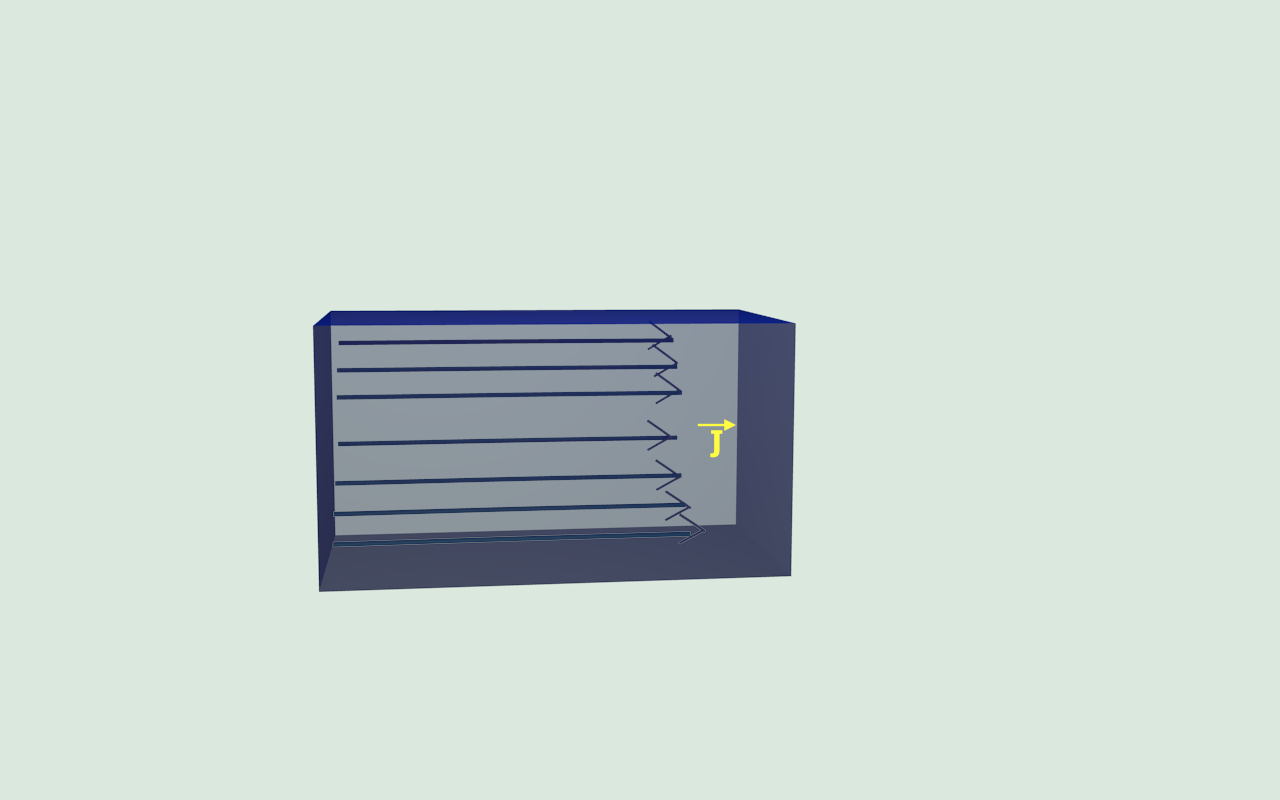
\includegraphics[height = 7cm, keepaspectratio]{graphes/blender_cuve_champvec.png}
%		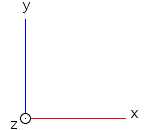
\includegraphics[height = 2cm, keepaspectratio]{graphes/axes.png}
		\caption{liquide faiblement ionisé soumis à un champ électrique $\vec{E}$, Blender}
		%		\end{subfigure}
	\end{center}
\end{figure}
\newline
On place un aimant de telle manière à générer un champ magnétique plus important sur une moitié du cube que l'autre.
\begin{figure}[!h]
	\begin{center}
	\centering
		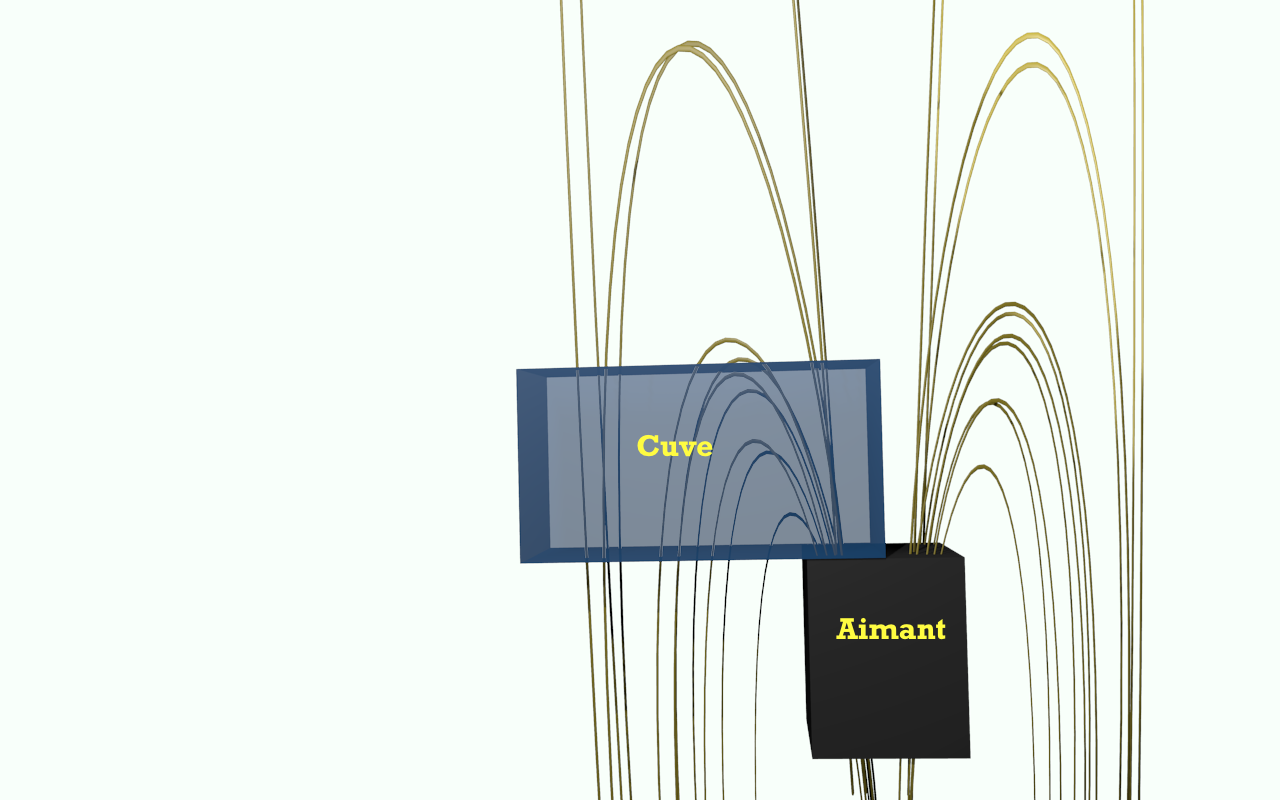
\includegraphics[height = 8cm, keepaspectratio]{graphes/blender_cuve_mag2.png} 
		%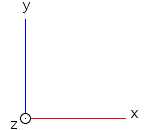
\includegraphics[height = 2cm, keepaspectratio]{graphes/axes.png}
		\caption{lignes de champ magnétique, Blender}
	\end{center}
\end{figure}
\newpage
La force magnétique $\vec{f_l}=\vec{j_0}\land\vec{B}$ permet ainsi de générer un tourbillon.\newline
\begin{figure}[h]
	\begin{center}
	\centering	
%	\begin{subfigure}[b]{0.3\textwidth}
%		\end{subfigure}
%		\begin{subfigure}[b]{0.3\textwidth}
		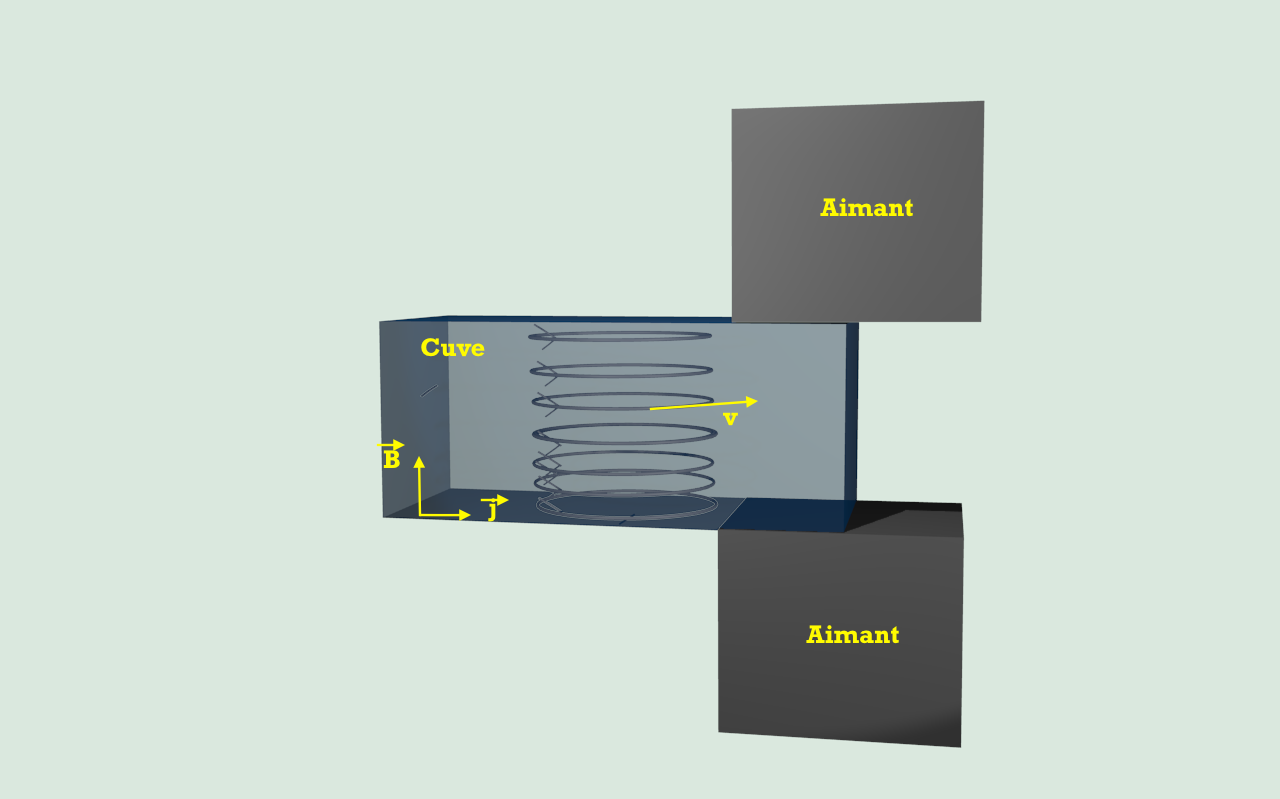
\includegraphics[height = 10cm, keepaspectratio]{graphes/blender_cuve_champvec2.png}
%		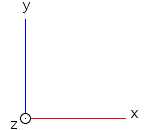
\includegraphics[height = 2cm, keepaspectratio]{graphes/axes.png}
		\caption{liquide faiblement ionisé soumis à un champ électrique et un champ magnétique $\vec{B}$, Blender}
%		\end{subfigure}
	\end{center}
\end{figure}
Afin de générer deux tourbillons, on place deux aimants l'un en face de l’autre sur le deuxième tiers du parallélépipède pour créer un champ B~ vertical sur le tiers au milieu.
On place aussi deux électrodes sur les faces opposées du parallélépipède pour créer un courant uniforme de densité $\vec{j}$.
Une force de Laplace est générée, due a` la difference de potentiel (P1 - P0) en présence d’un champ magnétique $\vec{B}$, deux tourbillons sont alors générés dans le parallélépipède
%Pour obtenir la situation de 3 tourbillon dans une cuve avec 2 parallèles er le dernier perpendiculaires aux 2 autres, nous allons utiliser un liquide faiblement conducteur soumis à un champ électrique est à des champs magnétiques pour créer les tourbillon : On place trois aimants pour générer les trois tourbillons créant ainsi un mouvement d'advection chaotique.


\begin{figure}[!h]
	\begin{center}
	\centering
		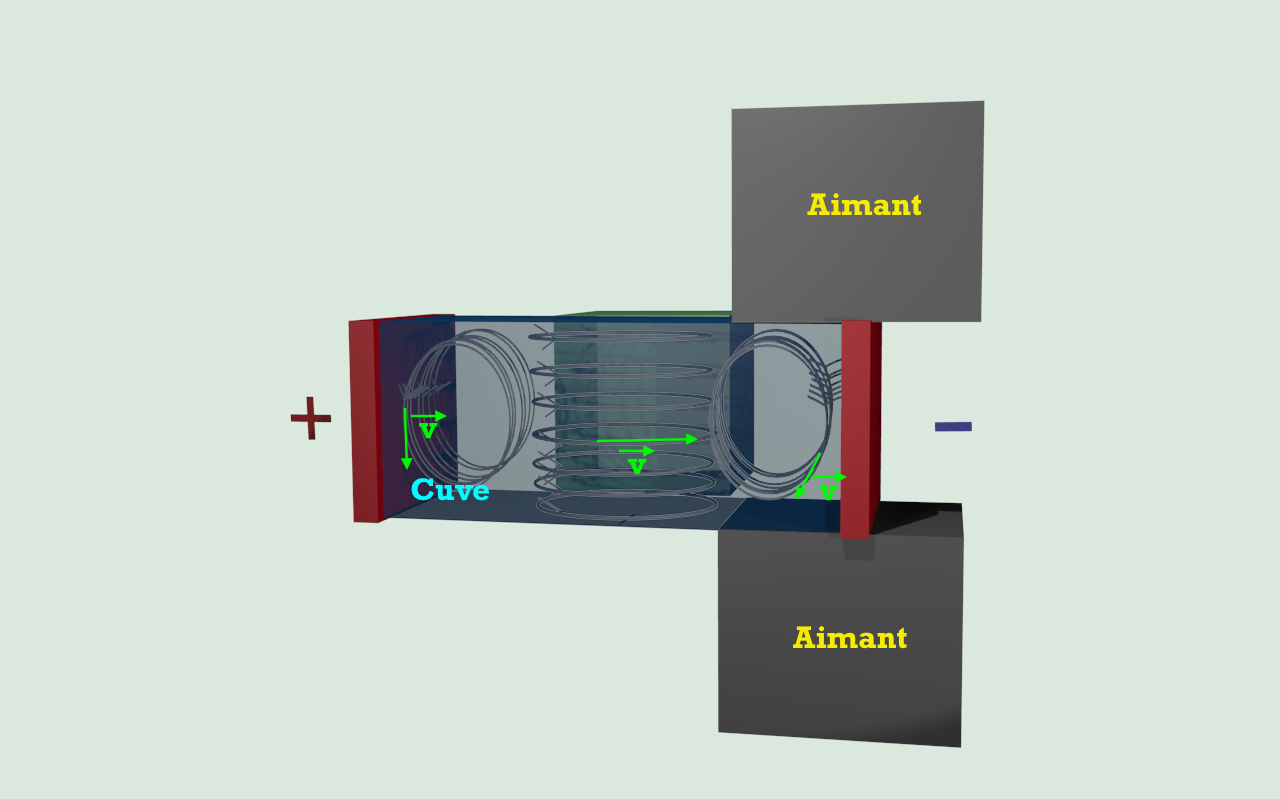
\includegraphics[height = 10cm, keepaspectratio]{graphes/blender_cuve_champvec3.png} 
		%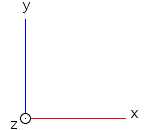
\includegraphics[height = 2cm, keepaspectratio]{graphes/axes.png}
		\caption{configuration avec 2 tourbillons, Blender}
	\end{center}
\end{figure}
\newpage

\subsection{hypothèses de modélisation}
Nous devons d'abord modéliser notre système , car dans les cas de système faisant intervenir des équations à dérivées partielles , la bonne définition du système est primordiale, avec notamment les conditions aux limites.\\
Notre système \{fluide\} sera modélisé par un fluide à faible nombre de Reynolds (visqueux) incompressible régi par les équations de Stokes que nous poserons dans le chapitre suivant. La densité de courant $\vec{j_0}$ est supposé uniforme sur le fluide.


%=====================================================================================================================================
%												CHAPITRE 1 CALCUL DU CHAMP MAGNETIQUE
%==========================================================================================================================================================
\newpage
\chapter{Modélisation du champ Magnétique de l'aimant}

Nous allons nous intéresser en premier lieu à modéliser le champ magnétique d'un aimant pour pouvoir obtenir à terme les forces de Laplace s'exerçant sur le fluide pour caractériser l'écoulement.

Nous cherche ainsi à modéliser le champ d'induction magnétique $\vec{B}(x,y,z)$ induit par un aimant (Figure 1). L'objectif sera d'abord de déterminer le champ magnétique dans une configuration quelconque, pour ensuite exploiter ces résultats et les employer dans la résolution numérique de Navier Stokes. \\
\begin{figure}[h]
\begin{center}
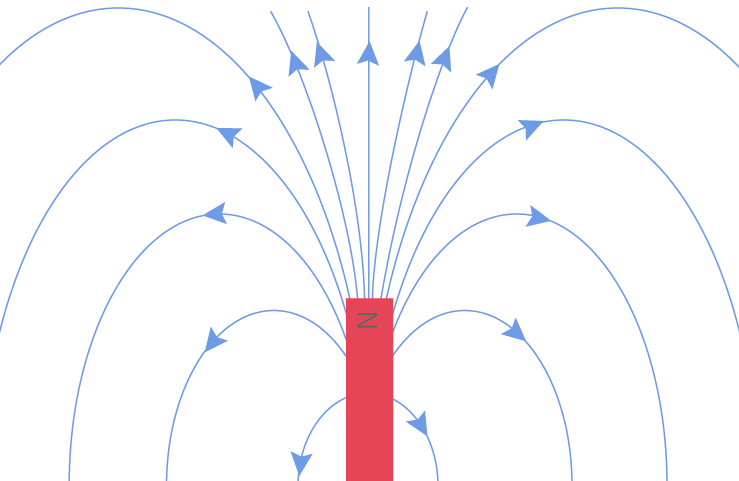
\includegraphics[height =4 cm, keepaspectratio]{graphes/champ_aimant1.png} %on affiche figure aimant
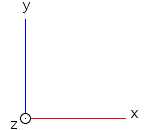
\includegraphics[height = 2cm, keepaspectratio]{graphes/axes.png}
\caption{champ magnétique d'un aimant coupe 2D}
\label{figure 1}
\end{center}
\end{figure}

On suppose que l'aimant à une longueur suffisante selon $\vec{z}$ pour être considéré comme infini selon l'axe $\vec{z}$.
On en déduit donc par le principe de Curie que le champ magnétique est invariant par translation selon $\vec{z}$. 
Ainsi \[\vec{B}(x,y,z) = \vec{B}(x,y)\]

On modélise donc le champ magnétique en deux-dimensions dans cette partie, dans la suite nous considérerons que le champ d'induction aura la même valeur selon la troisième dimension.
%======================= Mise en forme du probleme ================================================== 
\section{Mise en forme du problème}

Nous allons rechercher une solution du champ magnétique dans le domaine de résolution $\Omega$ (figure 2), $\Omega \subset R^{2}$. \\
\begin{figure}[h]
\begin{center}
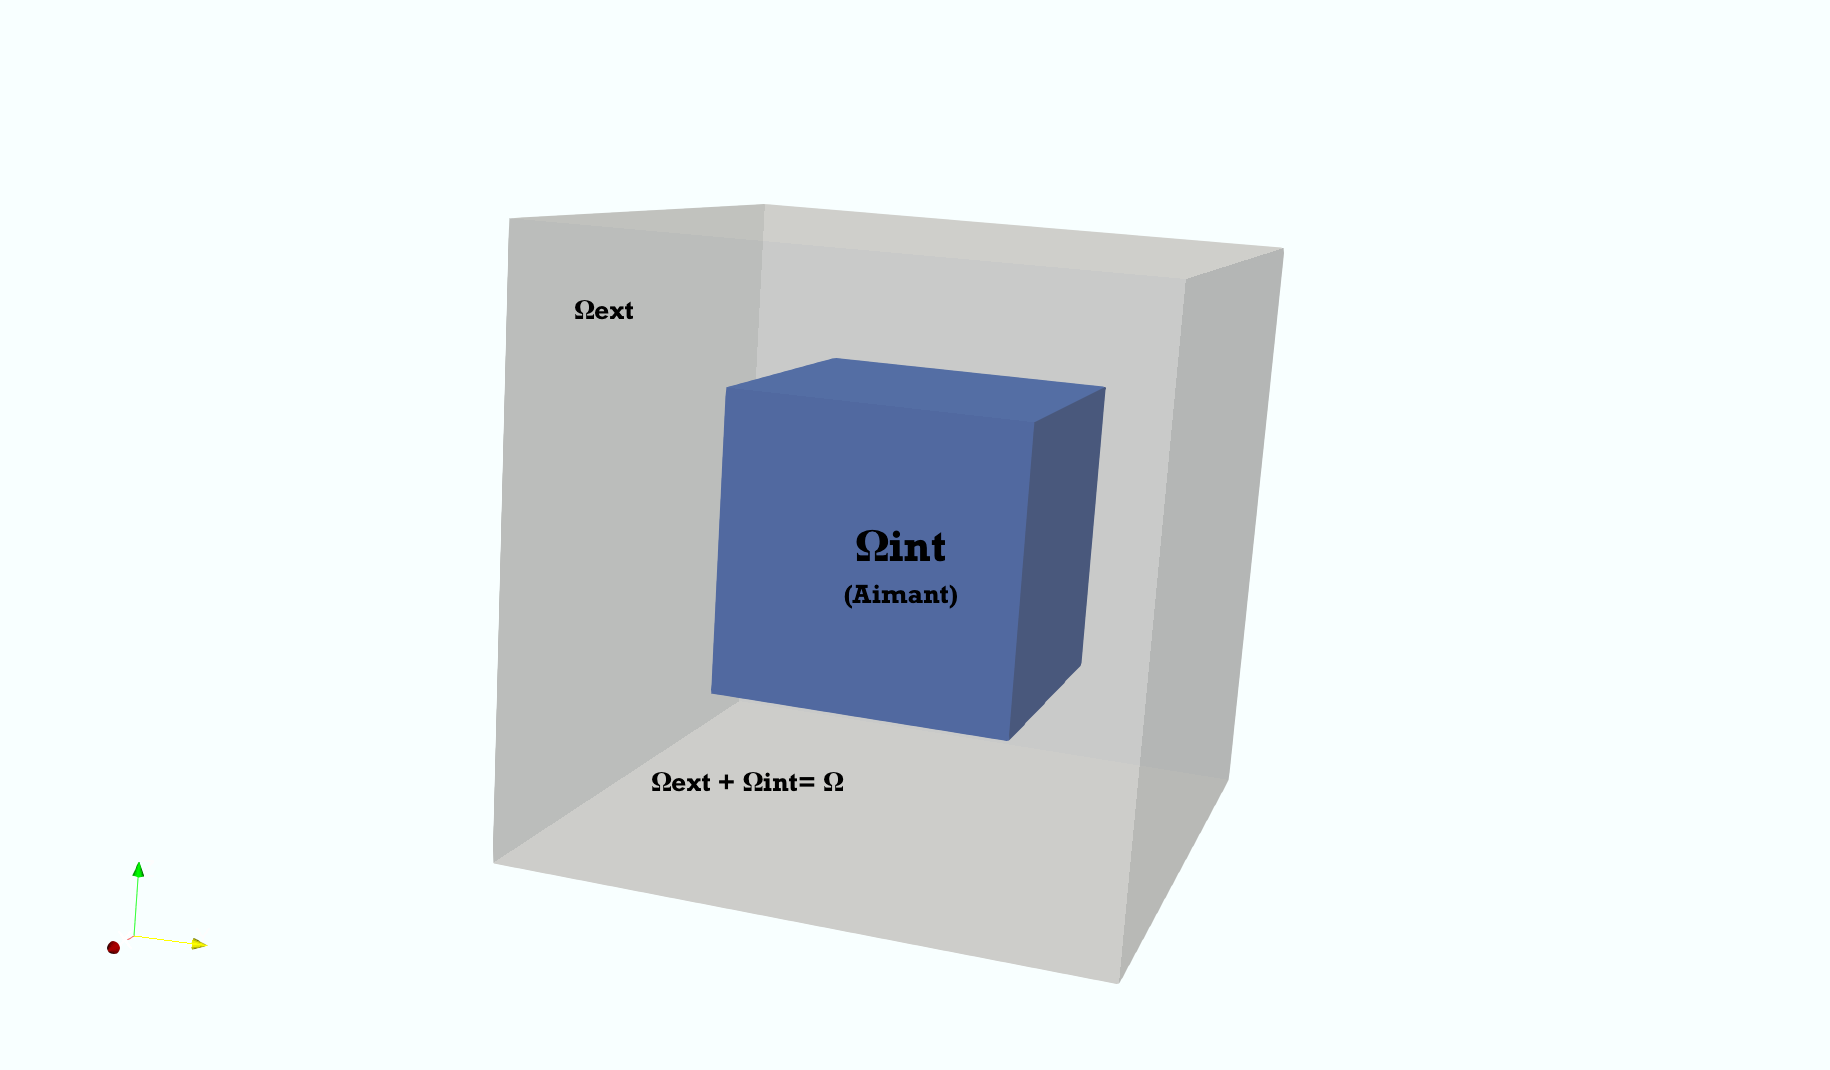
\includegraphics[height = 8cm, keepaspectratio]{graphes/Espacedetravail.png} 
\caption{domaines de résolution du problème, Blender}
\label{figure 2}
\end{center}
\end{figure}
On définit $\Omega_{int}$ le domaine de l'aimant, et $\Omega_{e}$ le domaine extérieur à l'aimant. 
\[\Omega_{e} = \Omega_{int} - \Omega\]

\newpage
On se place dans le régime stationnaire comme il n'y a pas de mouvements de l'aimant. \\
Le champ d'induction magnétique $\vec{B}$ est la somme du champs magnétique $\vec{H}$.

\[\vec{B}=\mu _{0}(\vec{H}+\vec{M})\]
$\mu _{0}$ est la perméabilité magnétique du vide. \\
L'aimantation $\vec{M}$ est nulle en dehors de l'aimant.
 
\[ 
\left\{
\begin{array}{ccc}
\begin{aligned}
	\vec{M} &= \vec{0} \  \text{dans} \ \Omega_{e} \\ 
	\vec{M} &= \vec{M_{0}} = \text{constante}  \ \text{dans}  \  \Omega_{\text{int}}
\end{aligned}
\end{array}
\right.
\]

Pour trouver le champ magnétique, on appliquer les équations fondamentales de la magnétostatique. L'équation de Maxwell nous donne 
\[
	\left\{
	\begin{array}{ccc}
	\begin{aligned}
		\Rot{\vec{H}} &= \vec {0} \\
		\Div{\vec{B}} &= 0
	\end{aligned}
	\end{array}
	\right.
\]

Le domaine étant simplement connexe, $\vec{H}$ dérive d'un potentiel $u$	.
\[
	\left\{
	\begin{array}{ccc}		
	\begin{aligned}
		\vec{H} &= \Grad{\vec{u}} \\
		\vec{B} &= \mu_{0}\times(\vec{\Grad{u}}+\vec{M})
	\end{aligned}
	\end{array}
	\right.
\]

Au sens des distributions pour toute fonction $\varphi\ $  dans $D(\Omega)$	
\[<\Div\vec{B},\varphi> \ = \ <-\vec{B},\vec{\Grad{\varphi}}>\]
On suppose $\vec{B} \in L^{3}_{1}(\Omega)$
\[<\Div\vec{B},\varphi> \ = \  -\int_{\Omega}\vec{B}. \vec{\Grad{\varphi}}\]
\[<\Div\vec{B},\varphi> \ = \ -\int_{\Omega}\mu_{0}(\vec{\Grad{u}}+\vec{M}) .{\Grad{\varphi}} = 0\]
Ainsi
\[\int_{\Omega}(\vec{\Grad{u}}+\vec{M}) . \vec{\Grad{\varphi}} = 0\]
Et comme $\vec{M}$ est nul en dehors du domaine $\Omega_{\text{int}}$ de l'aimant, on obtient (1)

On reconnait un problème de Dirichlet homogène qui admet une unique solution dans $H_{0}^{1}(\Omega)$ d'après le théorème de Lax-Migram.
\begin{equation}
\label{E}
\forall \varphi\ \in \Omega, \ \int_{\Omega}\bigtriangledown u .\bigtriangledown{\varphi} = -\vec{M_{0}}. \int_{\Omega_{int}}\bigtriangledown\varphi
\end{equation}

Adimensionnons (1)				:
\[
	\forall \varphi\  \in \Omega,\  \frac{1}{|\vec{M}_{0}|}\int_{\Omega}\bigtriangledown u.\bigtriangledown \varphi
	= -\vec{e}_{y}.\int_{\Omega_{int}}\bigtriangledown \varphi
\]
On prend pour la suite \[U =  \frac{u}{|\vec{M}_{0}|}  \] ce qui nous donne \[\vec{H^*} =\frac{\vec{H}}{M_0} \]
On établit ainsi \label{A}

\begin{equation}
\boxed{
\label{A}
	\forall \varphi\  \in \Omega,\ \int_{\Omega}\bigtriangledown U.\bigtriangledown \varphi
	=- \vec{e}_{y}.\int_{\Omega_{int}}\bigtriangledown \varphi}
\end{equation}
\\

\section{Méthode des éléments finis}

\subsection{Le maillage}
On recherche une solution approchée de l'équation numériquement en passant de l'espace continu à un espace discret. \\
\\
On utilise la méthode des éléments finis en recherchant une solution dans l'espace 
$V_{h} = \{u \ | \ u \in P^{1}(\Omega^{2}), u \in H^{1}_{0}(R^{2})\}$. \\
\\
On introduit une triangulation $T_{h}$ en subdivisant $\overline{\Omega}$, de bord $\Gamma \ = \ \partial\Omega$. 
Cette triangulation vérifie les propriétés suivantes :
\\
\begin{itemize}
  \item l’intersection de deux triangles K de $T_{h}$ doit être réduite à un sommet commun,\\ à une arête commune et entière ou à l'ensemble vide
  \item l’aire des triangles ne doit pas être nulle
  \item tous les coins du bord $\Gamma$ sont des sommets de triangles K de $T_{h}$
\end{itemize}

Le maillage ainsi construit est tel que
\[
\overline{\Omega} \ = \ \bigcup_{K \in T_{h}} K 
\]
\begin{figure}[h]
\begin{center}
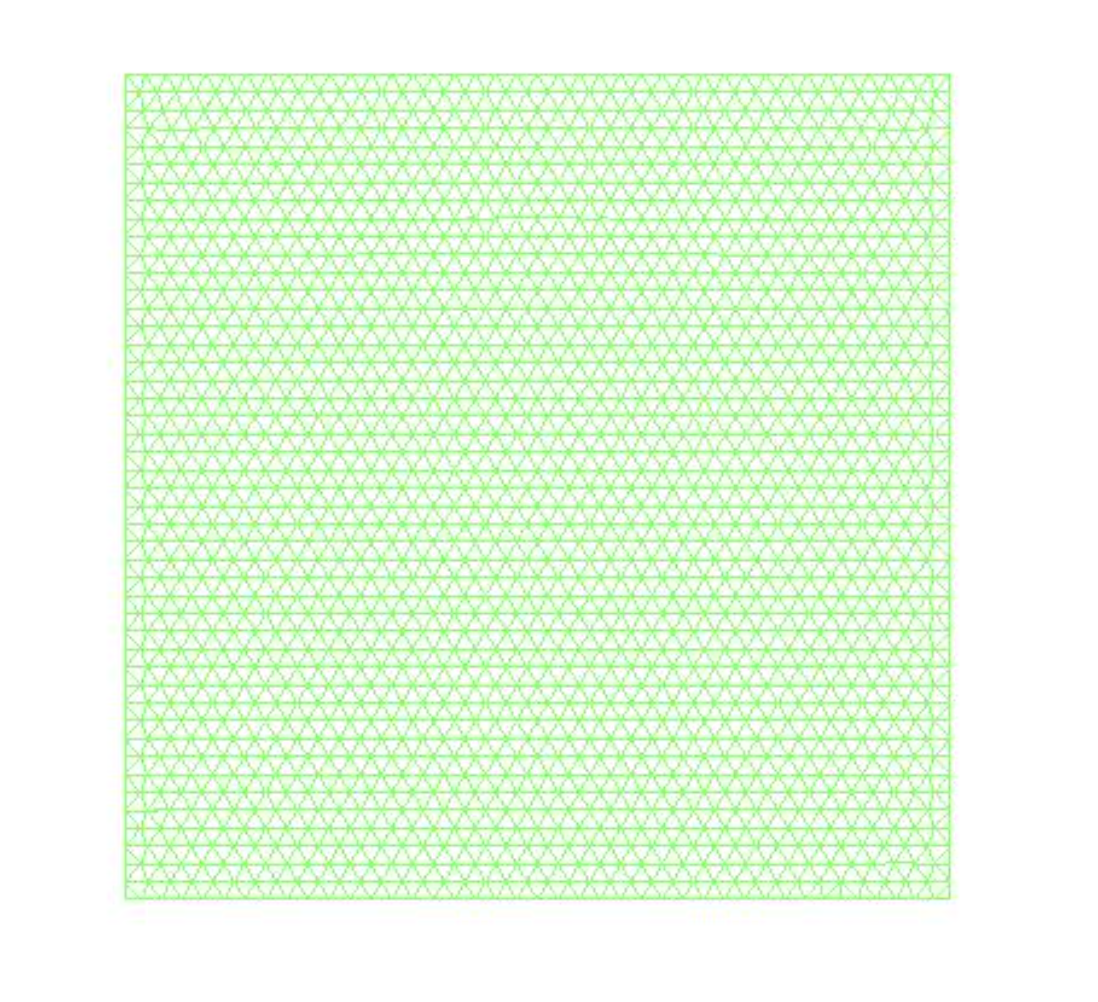
\includegraphics[height = 8cm, keepaspectratio]{graphes/Maillage_initial.png} 
\caption{\label{figure 3 } maillage effectué sur matlab à l'aide de mesh2D d'un carré 1$\times$1.05 avec un pas constant h = 0.1}
\end{center}
\end{figure}

On note que le maillage est caractérisé par la longueur de la plus petite arrête $h_{min}$ telle que 
\[
h_{min} \ = \ \min_{K \in T_{h}} h_{K}
\]
$h_{min}$ va notamment déterminer l'erreur entre la solution continue et la solution discrète.
On choisit une base de $V_{h}$, on prend la famille des fonctions de base  \\ $\varphi_{1}, \varphi_{2}, ..., \varphi_{N_{h}}$  telles qu'elles valent 1 en un sommet d’un triangle, et 0 pour tous les autres sommets. On note $P_{1},P_{2}, ..., P_{N_{h}}$ les sommets des triangles du maillage.
Les fonctions de base sont donc définies ainsi :
\[
\forall i,j \in [1, N_{h}]^{2} \ \varphi_{i} \in L^{2}(\Omega),\ \varphi_{i}(P_{j}) \ = \ \delta_{ij} \ \
\varphi_{i} \ = \ 0 \ sur \ \Gamma \]
Le support de $ \varphi_{i}$ est la réunion de tous les triangles ayant pour sommet $P_{i}$.\\
On vérifie que la famille ($\varphi_{1}, \varphi_{2}, ..., \varphi_{N_{h}}$) est une base de $V_{h}$.
Ainsi toute fonction g dans $V_{h}$ peut s'écrire comme une combinaisons linéaire des $\varphi_{i}$
\[
g = \sum_{i=1}^{N_{h}}{\ g_{i}\varphi_{i}} \text{ \ \ où } g_{i} = g(P_{i}),\  i= 1,2,...,N_{h}
\]

%=====================================================================================================
\subsection{Mise en équation}
%=======================================================================================================

Réécrivons (1.2) dans $V_{h}$ : 

\[
	\forall \varphi \in V_{h} , \ \int_{\Omega}\bigtriangledown u_{h}. \bigtriangledown \varphi = -\vec{M_{0}}. \int_{\Omega_{int}}\bigtriangledown \varphi
\]
Nous pouvons écrire $u_{h} = \sum_{i=1}^{N_{h}}{\ U_{i}\varphi_{i}} \text{ \ \ où } U_{i} = U(P_{i}),\  i= 1,2,...,N_{h}$ \\ et choisir $\varphi\ =\ \varphi_{i}$
ainsi
\[
	\int_{\Omega}\bigtriangledown u_{h}.\bigtriangledown \varphi\ 
	=\ 
	\sum_{i, j \in [1, N_{h}]^{2}} \int_{\Omega}u_{i}\bigtriangledown\varphi_{i}. \bigtriangledown\varphi_{j} 
	= 
	\sum_{i,j \in [1, N_{h}]^{2}} A_{ij} u_{i}
\]
avec A la matrice $N_{h} \times N_{h}$ de coefficients
\[
A_{ij}  = \int_{\Omega}\bigtriangledown\varphi_{i}.\bigtriangledown\varphi_{j}
\]
et si on introduit le vecteur $\vec{f}$ de composantes $f_{1},\ f_{2},..., f_{N_{h}}$ définies par
\[
f_{j} =  -\vec{e_{y}}.\int_{\Omega} \bigtriangledown\varphi_{j}
\]
Alors l'équation (2) revient de manière équivalente à résoudre le système linéaire 
\[
	A \times U =F
\]
 avec 
\[
U = 
\begin{pmatrix}
   u_{1} \\
   u_{2} \\
   \vdots \\
   u_{N_{h}}
\end{pmatrix}
\ \ F = 
\begin{pmatrix}
   f_{1} \\
   f_{2} \\
   \vdots \\
   f_{N_{h}}
\end{pmatrix}
\quad
A_{ij}  = \int_{\Omega}\bigtriangledown \varphi_{i}. \bigtriangledown \varphi_{j}
\]
On appelle A la matrice de rigidité.  \\

%================= passage element de reference =====================================================
\newpage
\subsection{Passage à un élément de référence}
Pour les calculer numériquement les matrices on utilise un triangle de référence normalisé $\hat{T}$. On passe du triangle $\Hat{T}$ à $T$ à l'aide de la transformation $F$. 
\begin{figure}[h!]
\begin{center}
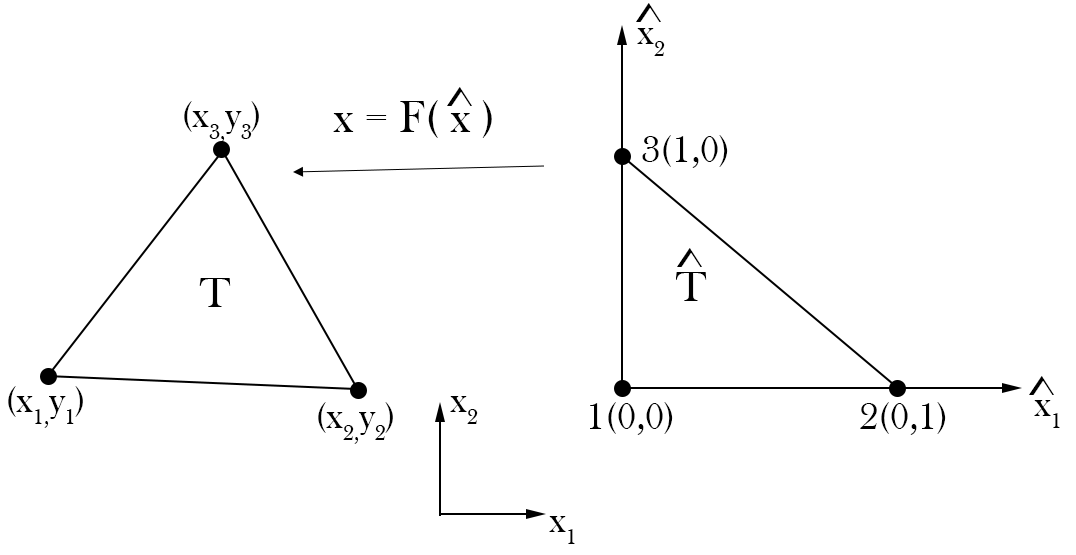
\includegraphics[height = 6cm, keepaspectratio]{graphes/transformation_de_maillage.png} 
\caption{\label{figure 4 } passage à un maillage de référence}
\end{center}
\end{figure}
On a pour le calcul du gradient de $\varphi_{i}$
\[ \bigtriangledown_{\hat{x}} \hat{\varphi} = (J)^{T} \bigtriangledown_{x} \varphi  \]
où J est la matrice Jacobienne de la transformation.
Calculons la matrice Jacobienne qui va dépendre des coordonnées $(x_{i},y_{i})$ des sommets pour chaque triangle.
\[
x = \begin{pmatrix}
   x_{1} \\
   x_{2} 
\end{pmatrix}
= \begin{pmatrix}
   F_{1}(\hat{x}) \\
   F_{2}(\hat{x}) 
\end{pmatrix}
= \begin{pmatrix}
   \hat{x}_{1} \\
   \hat{x}_{2} 
\end{pmatrix}
= J \times \hat{x} + C
\]
On obtient ainsi à l'aide d'un changement de variable le calcul de la matrice de rigidité (voir annexe A) : 
\[
\boxed{
\begin{aligned}
A_{ij} = 
	\iint_{\Omega}\bigtriangledown_{x}{\varphi_{i}} \bigtriangledown_{x}{\varphi_{j}} &= 
	\sum_{T \in \text{Supp}(\varphi_{i})\times \text{Supp}(\varphi_{j})}	
	\frac{\text{aire}(T)^{2}}{4}
	\begin{pmatrix}
   		y_{3}-y_{1} &  	x_{1}-x_{3}\\
   		y_{1}-y_{2} &  x_{2}-x_{1}
	\end{pmatrix}
	^{2}
	\bigtriangledown_{\hat{x}} \hat{\varphi_{i}}
	\bigtriangledown_{\hat{x}} \hat{\varphi_{j}}
\end{aligned}}
\]
\\
\\
Calculons à présent le terme source $f_{j} =  -\vec{e_{y}}.\int_{\Omega} \bigtriangledown\varphi_{j}$.
\\
\\
D'après Green-Ostrogradsky
\[
	\iint_{\Omega}\bigtriangledown_{x}{\varphi_{i}} =\ 
	\int_{\partial\Omega_{\text{int}}}\varphi_{i}.\vec{\text{n}} \ \partial s
\]

Ainsi	
\[
	\begin{aligned}
		\int_{\partial\Omega_{\text{int}}}\varphi_{i}.\vec{\text{n}}\ \partial s &= 
		\sum_{e \in \partial\Omega_{\text{int}}}\ \int_{e}\varphi_{i}.\vec{\text{n}}_{e}\ \partial s \\ &=  
		\sum_{e \in \partial\text{supp}(\varphi_{i})}\ \int_{e}\varphi_{i}.\vec{\text{n}}_{e}\ \partial s
	\end{aligned}
\]
où $\vec{\text{n}}_{e}$ est le vecteur unitaire normal sortant à l'arête e. \\
\begin{figure}[h]
\begin{center}
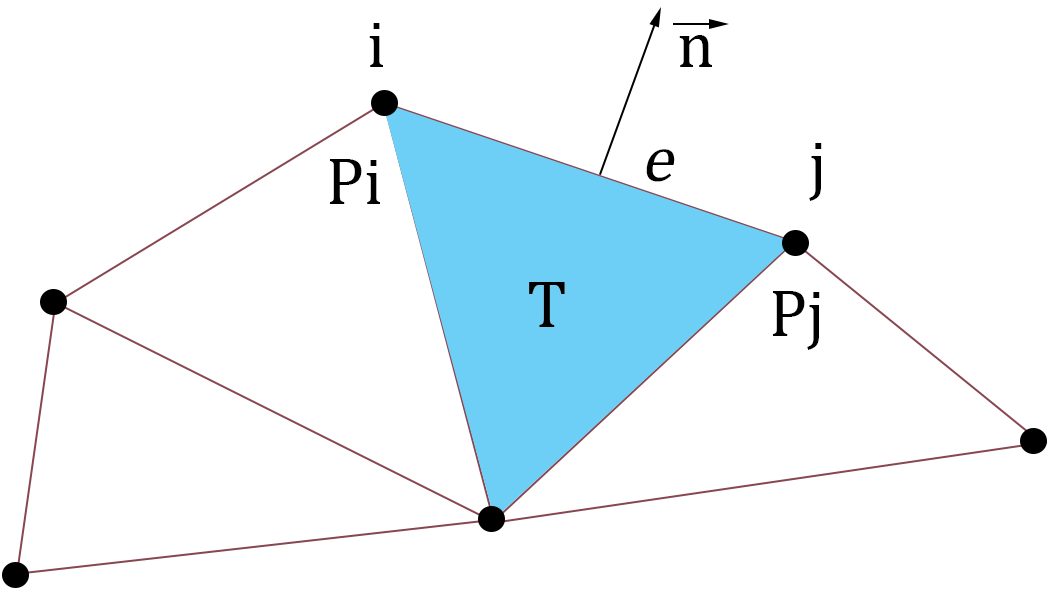
\includegraphics[height = 4cm, keepaspectratio]{graphes/bord.png}
\caption{arêtes}
\label{figure 1}
\end{center}
\end{figure}
\[
	|e|\times \vec{\text{n}}_{e}
	=
	\begin{pmatrix}
		y_{j}-y_{i} \\
		x_{i}-x_{j}
	\end{pmatrix}
\]
avec le changement de variable $x = s\times \text{Pi} + (1-s)\times \text{Pj}$,\ \ $s \in [0;1]$
\[
	\int_{e}\varphi_{i}.\vec{\text{n}}_{e}\ \partial s = |e|(\int_{0}^{1}\varphi_{i}\ \partial x ).\vec{\text{n}}_{e}
\]
avec 
\[
	\int_{0}^{1}\varphi_{i}\ \partial s  = \text{aire du triangle rectangle de coté |e| et de hauteur 1} = \frac{|e|}{2}
\]
d'où
\[
	\int_{e}\varphi_{i}.\vec{\text{n}}_{e}\ \partial s =
	|e|(\int_{0}^{1}\varphi_{i}\ \partial x ).\vec{\text{n}}_{e} =
	\frac{|e|}{2}.\vec{\text{n}}_{e} = 
	\frac{|e|^{2}}{2}
	\begin{pmatrix}
		y_{2}-y_{1} \\
		x_{1}-x_{2}
	\end{pmatrix}	
\] 
Au final
\[
	\iint_{\Omega}\bigtriangledown_{x}{\varphi_{i}} =
	\sum_{e \in \partial \text{supp}(\varphi_{i})}\ \int_{e}\varphi_{i}.\vec{\text{n}}_{e}\ \partial s =
	\sum_{e \in \partial\text{supp}(\varphi_{i})}
	\frac{|e|}{2}
	\begin{pmatrix}
		y_{2}-y_{1} \\
		x_{1}-x_{2}
	\end{pmatrix}
\]
\[
	\iint_{\Omega}\bigtriangledown_{x}{\varphi_{i}} =
	\sum_{e \in \partial \text{supp}(\varphi_{i})}
	\frac{|e|}{2}
	\begin{pmatrix}
		x_{2}-x_{1} \\
		y_{1}-y_{2}
	\end{pmatrix}
\]
Au final 
\[\boxed{f_{j} =  -\vec{e_{y}}.\sum_{e \in \partial \text{supp}(\varphi_{i})}
	\frac{|e|}{2}
	\begin{pmatrix}
		x_{2}-x_{1} \\
		y_{1}-y_{2}
	\end{pmatrix}}
\]

				

%====================== Calcul du gradient =========================================================							
\subsection{Calcul du Gradient}

Les calculs précédents nous permettent de trouver après résolution le potentielle $u$, ce que nous voulons obtenir à l'issue de notre étude est le champ d'induction magnétique $\vec{B}$ que l'on trouve par $\vec{B}= \bigtriangledown u$.
\\
\newline  On écrit la forme variationnelle dans $V_{h}$ (ainsi $\vec{B}$ suit une décomposition dans $V_h$, tel que $\vec{B}=\sum_{i} B_{xi}\varphi_i:$

\[
\begin{aligned}
		\forall \varphi \in V_{h} , \ \int_{\Omega}B.  \varphi &= \int_{\Omega}\bigtriangledown u.\varphi  \\
		\sum_{i,j}\;  \sum_{T \in \text{Supp}(\varphi_{i})\times \text{Supp}(\varphi_{j})}B_{i}\int_{T} \varphi_i\varphi_j & =  \sum_{i}  \sum_{T \in \text{Supp}(\varphi_{i})\times \text{Supp}(\varphi_{j})} u_i \int_{T}\bigtriangledown\varphi_i\varphi_j  
\end{aligned}
\]
Nous pouvons écrire l'équation ci dessus sous forme matricielle, en introduisant les matrices M et C, définit de la façon suivante :
\[
		M_{ij}=\int_{T} \varphi_i.\varphi_j \ \text{appellé la matrice de masse}
\]
\[
		C_{ij}=\int_{T} \bigtriangledown\varphi_i.\varphi_j 
\]
L'équation devient ainsi un problème linéaire sous forme matricielle  
\[
	M \times B=C \times U
\] 

Soit 
\[
	\boxed{B =M\up{-1}\times C \times U}
\]
Calculons ainsi les termes de la matrice C:
\[
\begin{aligned}
C_{ij} &= \iint_{\Omega}\bigtriangledown\varphi_i\varphi_j dx      
       = \sum_{K\in supp\varphi_j}\bigtriangledown_K\varphi_i \iint_{K} \varphi_jdx \\
	 &= \sum_{K\in supp\varphi_j}(J\up{-1}_K)^{T}(\bigtriangledown_{\hat{K}} \hat{\varphi_i})\iint_{\hat{K}}  |J_{K}| \hat{\varphi_j}\hat{dx} \\
	&= \sum_{K\in supp\varphi_j}(J\up{-1}_K)^{T}|J_K| (\bigtriangledown_{\hat{K} }\hat{\varphi_i})\iint_{\hat{K}}  \hat{\varphi_j}\hat{dx}
\end{aligned}
\]
\[\boxed{C_{ij} =  \sum_{K\in supp\varphi_j}(J\up{-1}_K)^{T}|J_K| (\bigtriangledown_{\hat{K} }\hat{\varphi_i})\iint_{\hat{K}}  \hat{\varphi_j}\hat{dx}} \]

Nous allons calculer pour l'implémentation algorithmique des matrice élémentaires qui vont regrouper sur chaque triangle les contributions croisés des trois nœuds, soit neuf termes dans chaque matrice élémentaire.
\newline
Calculons une matrice élémentaire de C sur un triangle K du maillage qui aura donc pour composantes (si on se place selon la composante x du gradient ) 

\[
|J_K| \times
\begin{pmatrix}
   	\bigtriangledown_{\hat{K} }{\varphi_1}_{|x}\iint_{\hat{K}}  \hat{\varphi_1}&\bigtriangledown_{K}{\varphi_1}_{|x}\iint_{\hat{K} } \hat{\varphi_2} &\bigtriangledown_{K}{\varphi_1}_{|x}\iint_{\hat{K} } \hat{\varphi_3}\\ 
  \bigtriangledown_{K }{\varphi_2}_{|x}\iint_{\hat{K }} \hat{\varphi_1} & \bigtriangledown_{K }{\varphi_2}_{|x}\iint_{\hat{K} }\hat{\varphi_2} & \bigtriangledown_{K }{\varphi_2}_{|x}\iint_	{\hat{K} } \hat{\varphi_3} \\
  \bigtriangledown_{K }{\varphi_3}_{|x}\iint_{\hat{K} } \hat{\varphi_1}&\bigtriangledown_{K }{\varphi_3}_{|x}\iint_{\hat{K} } \hat{\varphi_2} & \bigtriangledown_{K}{\varphi_3}_{|x}\iint_{\hat{K} } \hat{\varphi_3}
\end{pmatrix} 
\]
Calculons les intégrales :


\[	
  \left\{
    \begin{aligned}
      \iint_{\hat{K}} \hat{\varphi_1}{\hat{dx}} &= \int_{0}^{1}\int_{0}^{1-{\hat{x}}_2} (1-{{\hat{x}}_1}-{{\hat{x}}_2}) \hat{dx}_1 \hat{dx}_2 &=1/6\\
      \iint_{\hat{K} } \hat{\varphi_2}\hat{dx} &= \int_{0}^{1}\int_{0}^{1-{\hat{x}}_2} {{\hat{x}}_1} \hat{dx}_1 \hat{dx}_2 =1/6\\
       \iint_{\hat{K} } \hat{\varphi_3}\hat{dx} &= \int_{0}^{1}\int_{0}^{1-{\hat{x}}_2} {{\hat{x}}_1} \hat{dx}_1 \hat{dx}_2 =1/6\\
    \end{aligned}
  \right.
\]
\newpage
On a ainsi a matrice élémentaire du terme C sur un triangle K:

\[
\frac{1}{6}\times
	\begin{pmatrix}
   		\bigtriangledown_{K}{\varphi_1}_{|x} & \bigtriangledown_{K}{\varphi_1}_{|x} &  										    
   		\bigtriangledown_{K} {\varphi_1}_{|x} \\ 
    	\bigtriangledown_{K }{\varphi_2}_{|x} & \bigtriangledown_{K }{\varphi_2}_{|x} &  
    	\bigtriangledown_{K }{\varphi_2}_{|x} \\    										        
    	\bigtriangledown_{K}{\varphi_3}_{|x} & \bigtriangledown_{K}{\varphi_3}_{|x} & \bigtriangledown_{K}{\varphi_3}_{|x} \\ 
    \end{pmatrix} 
\]
\newline
Calculons également directement les matrices élémentaires pour la matrice de masse M définis par :
\[
M_{ij}=\iint_\Omega \varphi_i \varphi_j
\]
Sur un triangle K du maillage , on obtient de la même manière que précédemment 
\[
  \left.
    \begin{aligned}
		M_{ij}\up{K}=\int_0^{1}\int_0^{1-{\hat{x}}_2}|J_K|\hat{\varphi_i}(\hat{x})\hat{\varphi_j}(\hat{x})d\hat{x}\\
		=2\times\text{aire}(K)\times\int_0^{1-{\hat{x}}_2}\hat{\varphi_i}(\hat{x})\hat{\varphi_j}(\hat{x})d\hat{x}
    \end{aligned}
  \right.
\]
Il suffit donc de calculer les intégrales 
\[
	\int _0^{1}\int_0^{1-{\hat{x}}_2}\hat{\varphi_i}(\hat{x})\hat{\varphi_j}(\hat{x})d\hat{x}
\]
\\
par symétrie 
\[
	\forall i \int _0^{1}\int_0^{1-\hat{x}_{2}}\hat{\varphi_i}\up{2}= \int _0^{1} \int_0^{1-\hat{x}_{2}}\hat{x}_{2}^{2}d\hat{x}_{1}d\hat{x}_{2}=\frac{1}{12}
\]
\\%
\[
	\forall i \neq j \int _0^{1}\int_0^{1-{\hat{x}}_2}\hat{\varphi_i} \times \hat{\varphi_j}=\int _0^{1} \int_0^{1-\hat{x}_{2}}\hat{x}_{1}\hat{x}_{2}d\hat{x}_{1}d\hat{x}_{2}=\frac{1}{24}
\]
\\%
On en déduit la matrice de masse élémentaire sur un triangle de maillage 
\\%
\[
	\boxed{M\up{K}=\frac{\text{aire}(K)}{12}\times 
	\begin{pmatrix}
   		2 & 1 & 1 \\
   		1 &  2 & 1 \\
   		1 &  1 & 2
	\end{pmatrix}}
\]

%====================== Algorithme Matlab ======================================================= 
\subsection{Implémentation algorithmique}

Pour la résolution du problème nous utiliserons matlab avec la bibliothèque Mesh2D par Darren Engwirda pour la création du maillage 2D.
La résolution est effectué sur un maillage $5\times 5$ avec en son centre un aimant de taille $1\times 1$cm.

\begin{figure}[h]
	\begin{center}
	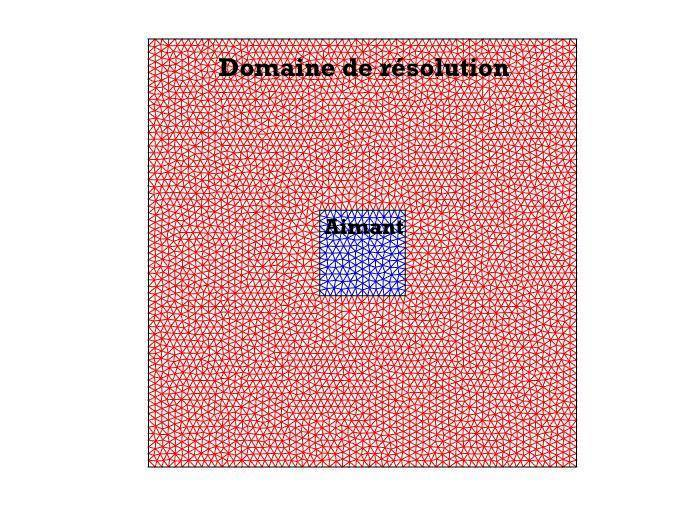
\includegraphics[height = 7cm, keepaspectratio]{graphes/maillage_resolution_champ_magnetique.jpg} 
	\caption{\label{figure 3 } maillage effectué sur matlab à l'aide de mesh2D dans la configuration décrite pour un pas h = 0.1}
	\end{center}
\end{figure}

Pour le calcul nécessaire des différentes matrice afin de résoudre le problème linéaire $A\times U = F$, les algorithmes reposent sur la même méthodologie de calcul :
Par exemple pour le calcul de la matrice A : 
\[
\begin{aligned}
A_{ij} = 
	\iint_{\Omega}\bigtriangledown_{x}{\varphi_{i}} \bigtriangledown_{x}{\varphi_{j}} &= 
	\sum_{T \in \text{Supp}(\varphi_{i})\times \text{Supp}(\varphi_{j})}	
	\frac{\text{aire}(T)^{2}}{4}
	\begin{pmatrix}
   		y_{3}-y_{1} &  	x_{1}-x_{3}\\
   		y_{1}-y_{2} &  x_{2}-x_{1}
	\end{pmatrix}
	^{2}
	\bigtriangledown_{\hat{x}} \hat{\varphi_{i}}
	\bigtriangledown_{\hat{x}} \hat{\varphi_{j}}
\end{aligned}
\]
Le principe consiste à ne pas recherche le support croisé des fonctions $\varphi_i$ et $\varphi_j$ (ce qui donnerait une complexité trop importante) mais à boucler sur les triangles et placer dans la matrice les contributions correspondantes à chacun de leurs nœuds avec leur indices. Notamment avec l'outil matriciel $sparse$ de matlab qui permet d'exploiter en temps de calcul et d'espace mémoire le fait que la matrice de rigidité A est creuse, comme pour deux fonction $\varphi_{i}$ et $\varphi_{j}$ l'intersection de leurs support se réduit à deux triangle.
\\
\\
Ainsi pour le calcul de A chaque triangle engendre une matrice élémentaire $ 3\times 3$ (car 3 nœuds pour chaque triangle donc 9 termes croisés) symétrique vu le calcul du terme $A_{ij}$ dont on place les terme dans la matrice A à chaque itération sur les triangles.
\\
\\Le principe est le même pour le terme source, pour chaque triangle appartenant au bord de l'aimant avec comme noeuds sur le bord les nœuds $\text{p}_{i}$ et  $\text{p}_{j}$ on place deux fois le même terme $\frac{|e|}{2}\begin{pmatrix} 
   									0 & 1\\
								\end{pmatrix}^{T}.
								\vec{\text{n}}_{e}$ 
(que l'on à calculé p.21) aux indices $\text{p}_{i}$ et  $\text{p}_{j}$ dans la matrice du terme source.
\\
\\
Et de même également pour le calcul des matrices M et C pour le gradient, dont nous avons explicité les matrices élémentaires.	

Voici une présentation succinte de l'algorithme de résolution, les fonctions utilisés sont détaillé dans l'annexe \ref{annexe_2}.

Pour la génération du maillage, on tulise la fonction meshfaces fournis par la bibliothèque Mesh2D par Darren Engwirda
\begin{verbatim}
 [v,t,fnum] = meshfaces(node,edge,face,hdata); %construction du maillage
 
 v : vecteur colonne regroupant les coordonnées des nœuds
 t : table de connectivité des triangle
 fnum : numéros de face des triangles du maillages (1 ou 2), 
 si sur le domaine des l'aimant ou de la cuve
\end{verbatim}
Calcul de la matrice de rigidité A et de la matrice de masse M : 
\begin{verbatim}
[M, nn, ibint, ic2] = matrixP1final(v,t,fnum,node1,edge1,node2,edge2);
[A]= matrixP1vect(v,t);
\end{verbatim}

On enlève les noeuds sur le bord du domaine de résolution comme la condition aux limite impose que $\Delta u = 0$ sur le bord, que nous considerons équivalente à $u = 0$ 
\begin{verbatim}
A1 = A1(ic2,ic2);	%ic2 sont les noeuds intérieurs du maillage
sol = A1\M;			%résolution linéaire
\end{verbatim}
Calcul du gradient de $u$ :
\begin{verbatim}
B = gradient(u,v,t);
 quiver(X,Y,B_X,B_Y);		%affichage du résultat final
\end{verbatim}

%====================== resultats  ===========================================================================
 
\subsection{Résultats de la simulation}

Voici les résultats de la simulation pour un maillage de pas 0.2 et de taille $5 \times 5$ pour un aimant de taille $1 \times 1$
\begin{figure}[!h]
\begin{center}
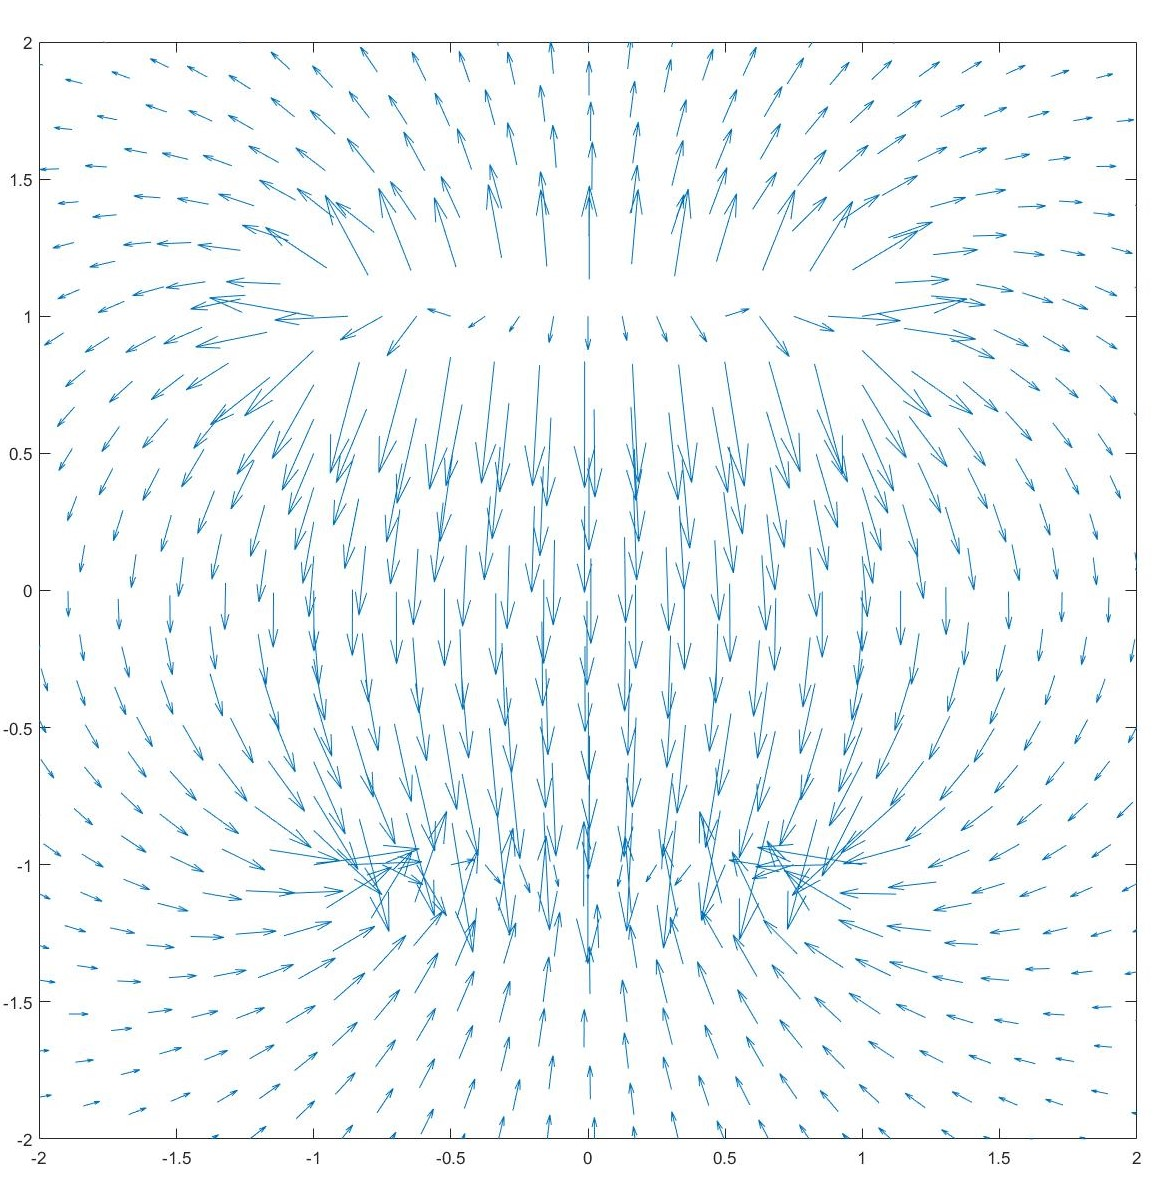
\includegraphics[height = 10cm, keepaspectratio]{graphes/resultat_champ.jpg}
\caption{affichage résolution centrée sur [-2, 2]}
\label{figure 1}
\end{center}
\end{figure}
On voit que les vecteurs suivent les dessin des lignes de champ que l'on peut attendre d'un aimant.
On peut s'inquiéter de la discontinuité des valeurs au bord de l'aimant mais ce la est en accord avec la formulation du champ d'induction comme la somme d'un champ d'excitation et d'une aimantation, nulle en dehors de l'aimant $\vec{B}=\mu _{0}(\vec{H}+\vec{M})$, d'où cette discontinuité que l'on observe.
\begin{figure}[!h]
\begin{center}
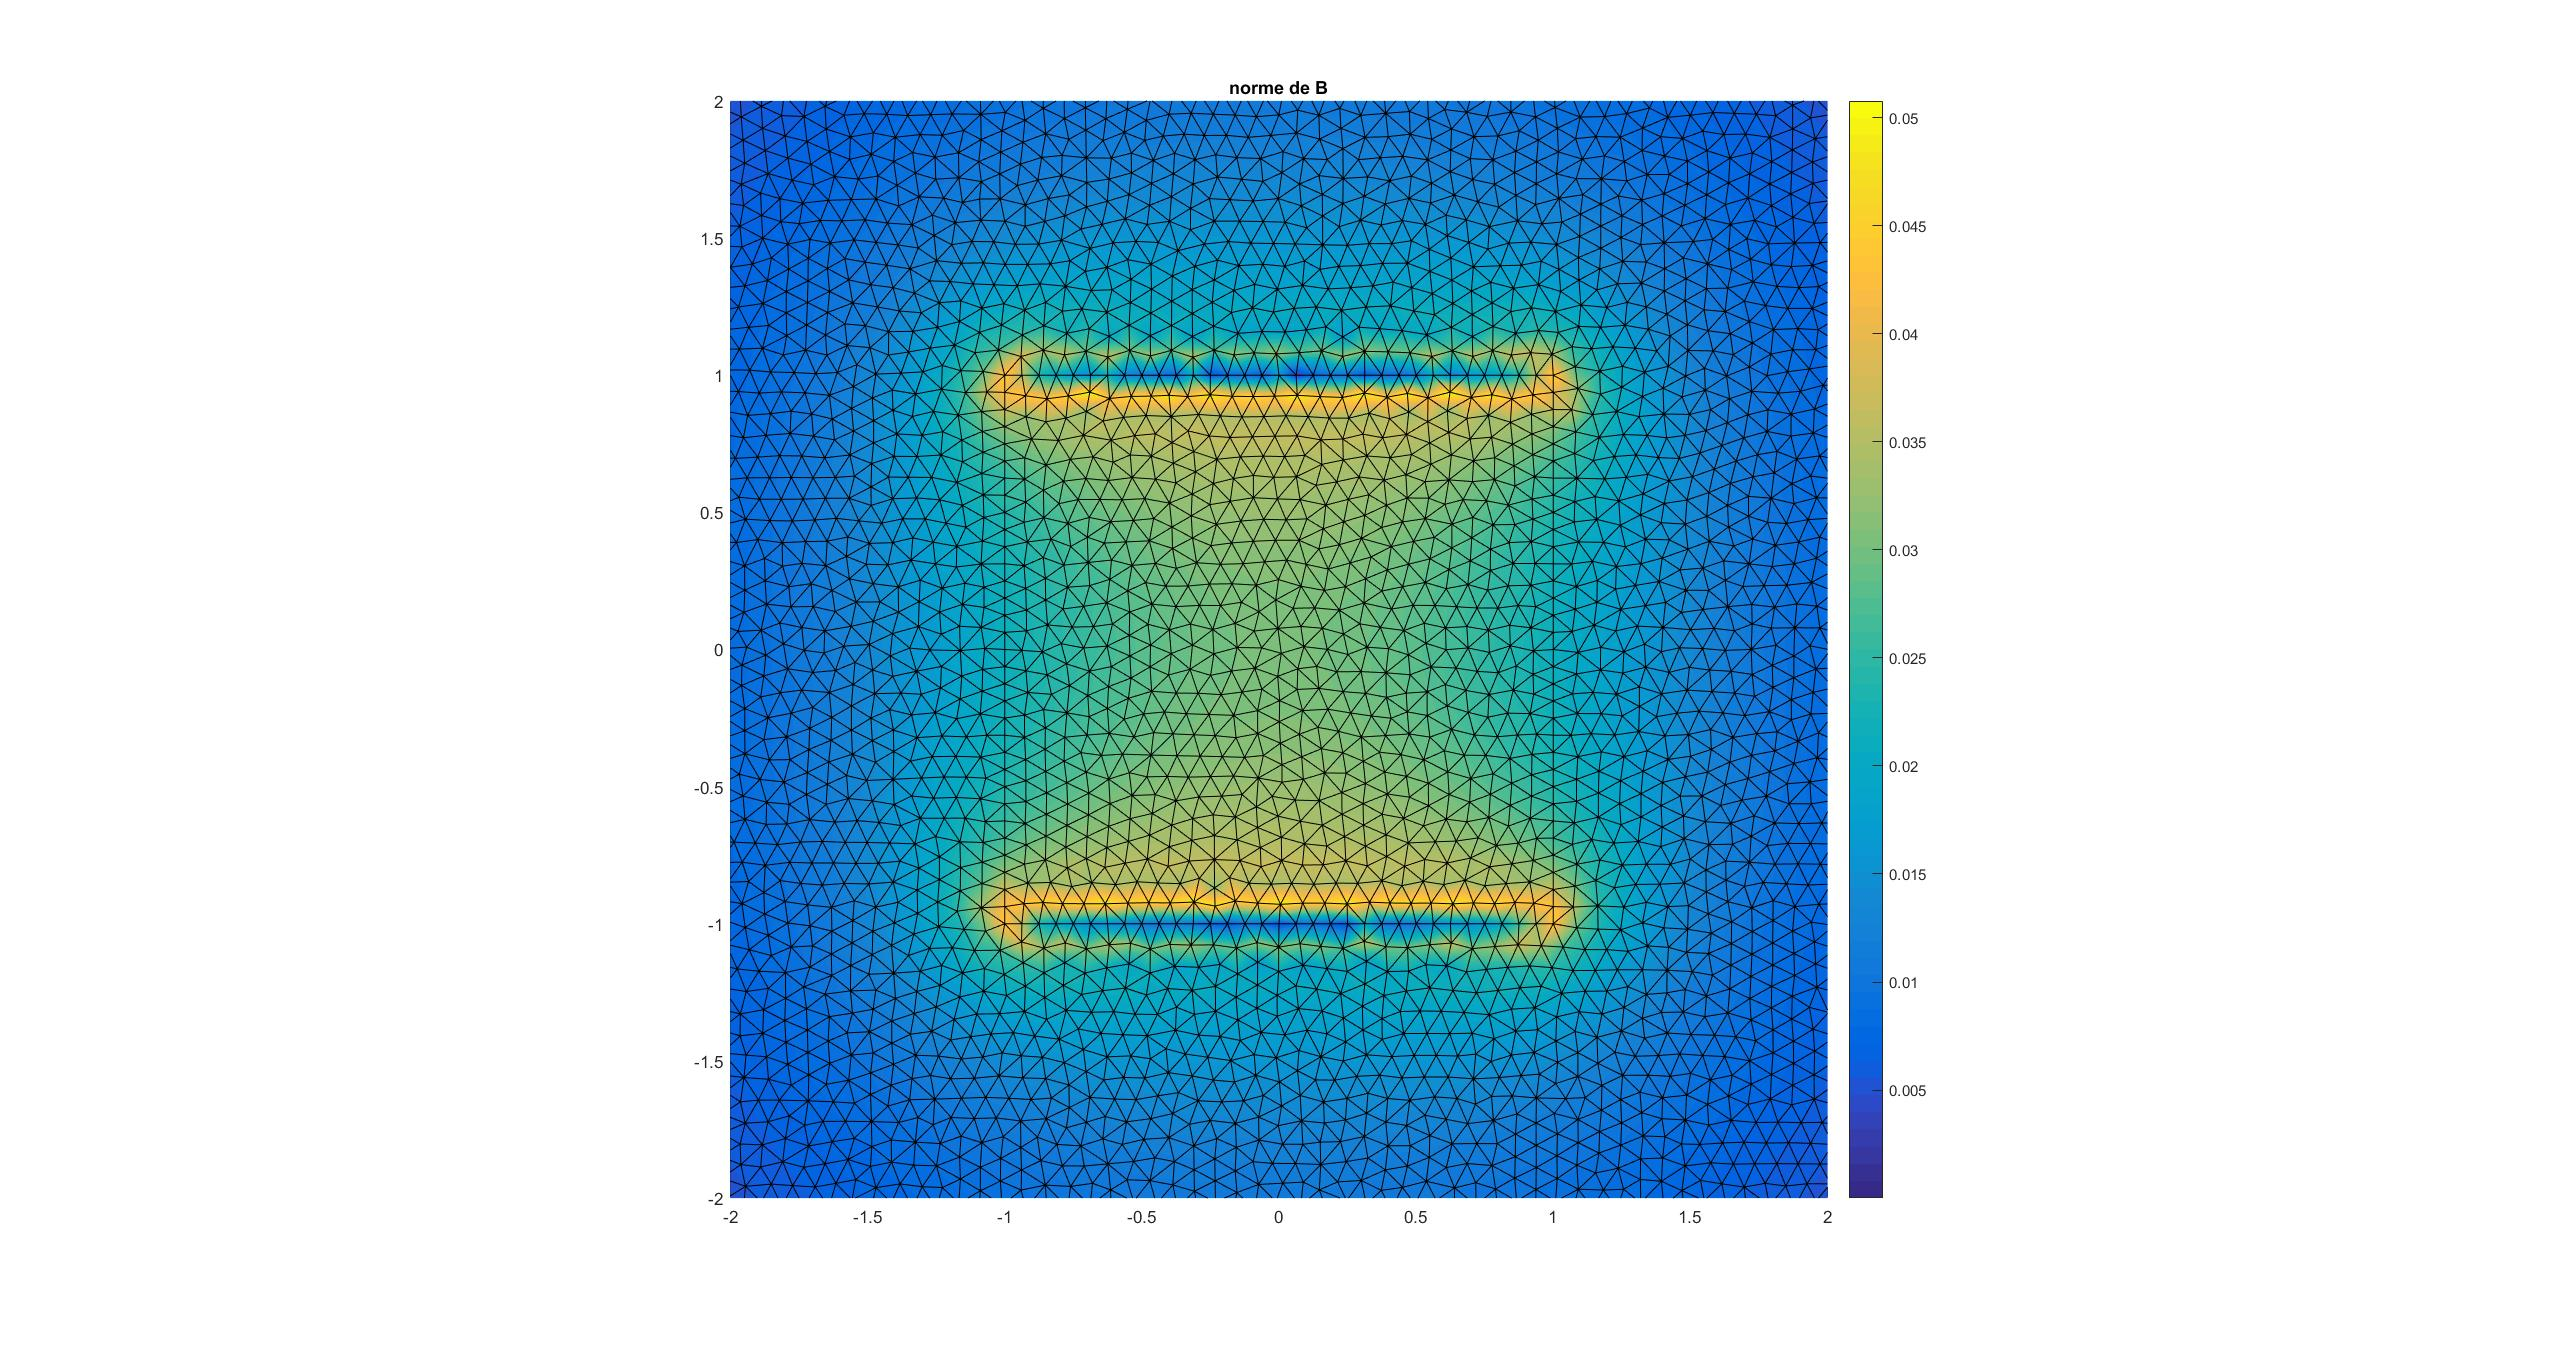
\includegraphics[height = 8 cm, keepaspectratio]{graphes/norme_du_champ.jpg}
\caption{affichage résolution centrée sur [-2, 2]}
\label{figure 1}
\end{center}
\end{figure}
%=========================================================================================================================================================
%												chapitre 2 equations de Navier_Stockes
%=========================================================================================================================================================
\newpage
\chapter{Équations de  Navier Stokes} 
Nous allons à présent nous intéresser à la modélisation de l'écoulement, qui suit les équations de Navier-Stokes d'après les hypothèses que nous avons émis précédemment. 
Nous supposons que nous avons à notre disposition deux aimants, qui sont perpendiculaires sur les côtés de la cuve, l'un produit un champ $B_1$, l'autre produit un champ $B_2$
Le premier aimant va produire un tourbillon dans le fluide, le deuxième va produire deux tourbillons parallèles, qui sont orthogonaux au premier tourbillon . Tout cela dans le but d'obtenir un écoulement tourbillonnaire. 
\begin{figure}[!h]
\begin{center}
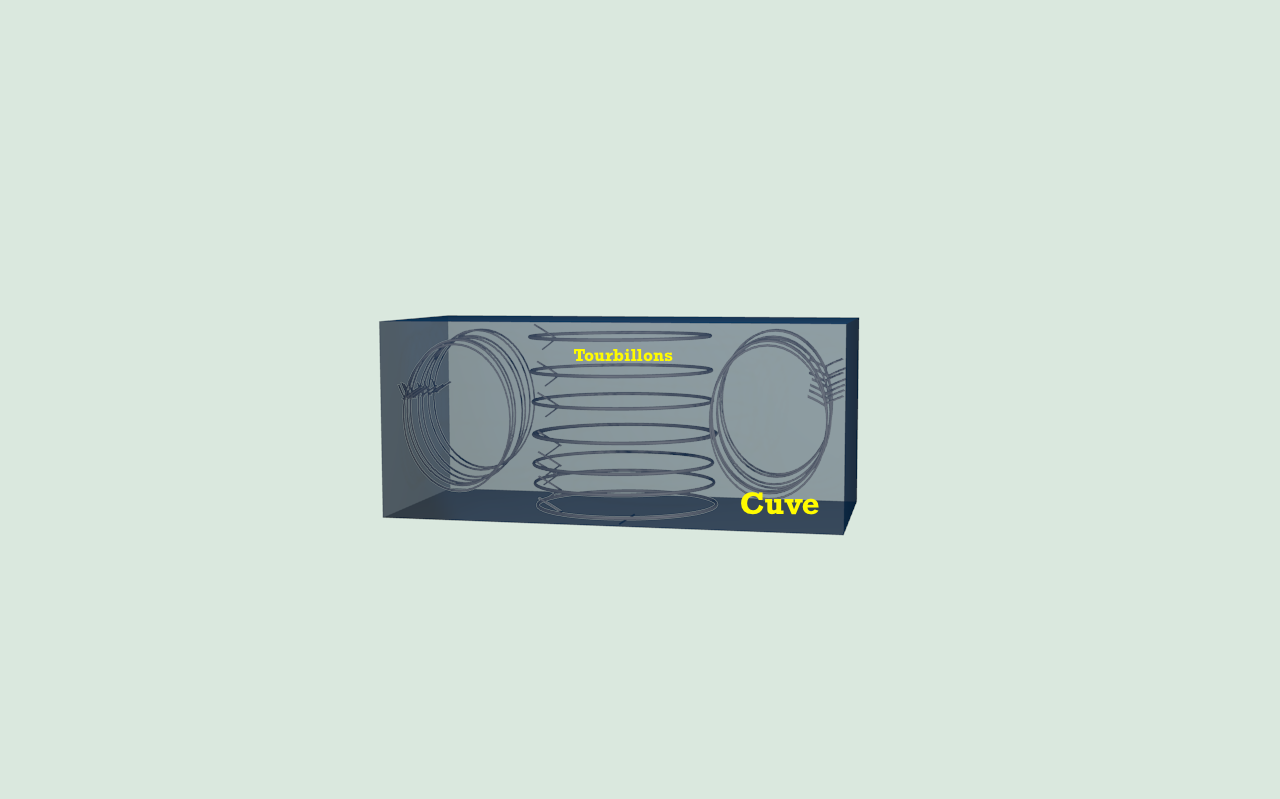
\includegraphics[height = 8 cm, keepaspectratio]{graphes/3_tourbillons.png}
\caption{les trois tourbillons que nous souhaitons obtenir avec notre dispositif expérimental}
\label{figure 1}
\end{center}
\end{figure}
%======================== Equations de Navier-stokes==========================================================
\newpage
\subsection{Équations de Stokes}

Le liquide est un conducteur placé dans un champ magnétique et parcouru par un courant supposé uniforme $\vec{j_0}$.
\normalsize 
Afin de pouvoir trouver l'équation de la trajectoire d’un point donné, on cherche tout d’abord à trouver la vitesse dans l'écoulement du fluide contenu dans un domaine $\Omega$.
\\A partir des équations de Navier-Stokes incompressibles, on détermine simultanément la vitesse  $V$ et la pression $P$. 
\\
\\
On émet les hypothèses suivantes :
\\
Dans un premier temps, nous pouvons négliger les forces d’inertie du fluide comme on a un faible nombre de Reynolds.
Le fluide visqueux est en mouvement le long d’une paroi solide fixe d’où une vitesse nulle sur le bord car 
$\vec{V_{\partial\Omega}}=\vec{V_{\text{paroi}}}=\vec{0}$
\\	
Finalement, on se place en régime stationnaire.
\begin{equation*}
  \left\{
    \begin{aligned}
      &\vec{0}=-\vec{\bigtriangledown}P +\mu\vec{\Delta}V +\vec{f}\;\text{dans }\Omega \\
      &\text{div}(\vec{V})=0\;\text{dans }\Omega \\     
      &\vec{V}=\vec{0}\;\text{sur }\partial\Omega
    \end{aligned}
  \right.
\end{equation*}

La force $\vec{f}$ correspond à la force de Laplace induite par le champ magnétique. La densité volumique de cette force est donnée par :
\[
\begin{aligned}
	\vec{f}=\vec{j_0}\land\vec{B}&=j_0\times M_0\times \vec{j}\wedge \vec{B^*} \\
	 \vec{B^*} =\frac{\vec{B}}{M_0}, 
	\ &\text{et} \ j_0=\frac{\Delta E}{L}\sigma
	\\
\text{avec} \quad
&\sigma : \text{la conductivité du fluide }
\\%
&\text{L: la longueur de base de la cuve} \\
&\Delta E : \text{la différence de potentiel}
\end{aligned} \\
\]
Ainsi on peut calculer la force magnétique pour un champ magnétique $\vec{B_1}$
\[
	\vec{B_1} = 
	\begin{pmatrix}
   		B_{1,x}\\
  		 B _{1,y}\\
  		 0
	\end{pmatrix} 
\]
\[
	\vec{f}=j_0\vec{e}_{x}
	\wedge\begin{pmatrix}
   		B_{1,x}\\
   		B _{1,y}\\
   		0
\end{pmatrix}=
j_0\times \begin{pmatrix}
  			0\\
   			0\\
    		B_{1,y}
			\end{pmatrix} 
\]

%==================================================== Adimensionnement de l'équation de Stokes ============================================================

\subsection{Adimensionnement de l'équation de Stokes}

\normalsize Afin de résoudre un seul système indépendamment des constantes, on adimensionne l'équation de Stokes. Le régime stationnaire sera pris en compte après adimensionnement.
\\%
Posons :
\begin{equation*}
\vec{V'}(x,t)=\frac{\vec{V}(x,t)}{V_0}\;;\vec{x'}=\frac{\vec{x}}{L_0}\; ; \vec{f'}(\vec{x'})=\frac{\vec{f}(\vec{x})}{j_0M_0}\;;P'=\frac{P}{P_0}\; ;t'=\frac{t}{\frac{L_0^2}{\mu}}\;
\end{equation*}
En injectant dans l'équation de Stokes d'évolution :
\begin{equation*}
  \left\{
    \begin{aligned}
    \rho\frac{\partial \vec{V}}{\partial t}=-\vec{\bigtriangledown} P + \mu \vec{\Delta}\vec{V}+\vec{f}
        \end{aligned}
  \right.
\end{equation*}
il en résulte :
\begin{equation*}
  \left\{
    \begin{aligned}
    \frac{\partial \vec{V'}}{\partial t}=-\frac{L_0 P_0}{\rho \mu V_0}\vec{\bigtriangledown} P '+  \vec{\Delta}\vec{V'}+\frac{L_0^2j_0M_0}{\mu V_0}\vec{f'}
        \end{aligned}
  \right.
\end{equation*}
On adimensionne par rapport à $V_0$ et $P_0$ de sorte que $\frac{L_0 P_0}{\rho \mu V_0}=1$ et $ \frac{L_0^2j _0M_0}{\mu V_0}=1$, le régime stationnaire étant établi:
\[
      \vec{0}=-\vec{\bigtriangledown}P' +\vec{\Delta}V' +\vec{f'}\;\text{dans }\Omega 
\]

%================= Formulation variationnelle =========================================================
\subsection{Formulation variationnelle}

Afin d'obtenir la formulation variationnelle de l'équation de Stokes, on passe dans l'espace des distribution de sorte que pour toute fonctions test $\varphi$ on a 
\[
	\int_\Omega\vec{\bigtriangledown}P'\times \vec \varphi=\int_\Omega-\mu\vec{\Delta}V'\times \vec \varphi +\int_\Omega\vec{f'}\times \vec \varphi 
\]
En appliquant la formule de Green, on obtient :

\[
\forall \varphi \in D(\Omega) \quad  \int_\Omega\vec{\bigtriangledown}P'. \vec \varphi + \int_{\Omega}\bigtriangledown V'. \bigtriangledown \varphi = \int_\Omega\vec{f'}. \vec \varphi
\]
Comme précédemment nous nous plaçons dans l'espace $V_{h}$ d'approximation polynomiale.
Nous pouvons ainsi décomposer les champs de pression $P'$, la vitesse $V'$ et la force $\vec{f'}$ dans la base des $(\varphi_{i})$:

\begin{equation*}
  \left\{
    \begin{aligned}
 &V '= \sum_{i=1}^{N_{h}}{\ V_{i}\varphi_{i}} \text{ \ \ où } V_{i} = V(P_{i}),\  i= 1,2,...,N_{h}\\
 &P '= \sum_{i=1}^{N_{h}}{\ P_{i}\varphi_{i}} \text{ \ \ où } P_{i} = P(P_{i}),\  i= 1,2,...,N_{h}\\
 &f' = \sum_{i=1}^{N_{h}}{\ f_{i}\varphi_{i}} \text{ \ \ où } f_{i} = f(P_{i}),\  i= 1,2,...,N_{h}\\
\end{aligned}
  \right.
\end{equation*}$ $ \\ 
On prend $\varphi\ =\ \varphi_{i}$ un vecteur de la base
\begin{equation*}
  \left\{
    \begin{aligned}
	&\int_{\Omega}\bigtriangledown V_{h}.\bigtriangledown \varphi\ 
	=\ 
	\sum_{i, j \in [1, N_{h}]^{2}} \int_{\Omega}V_{i}\bigtriangledown\varphi_{i}. \bigtriangledown\varphi_{j} 
	= 
	\sum_{i,j \in [1, N_{h}]^{2}} A_{ij} V_{i}\\
	&\int_{\Omega}\bigtriangledown P_{h}.\varphi\ 
	=\ 
	\sum_{i, j \in [1, N_{h}]^{2}} \int_{\Omega}P_{i}\bigtriangledown\varphi_{i}. \varphi_{j} 
	= 
	\sum_{i,j \in [1, N_{h}]^{2}}C_{ij} u_{i}\\
	&\int_{\Omega} f. \varphi\ 
	=\ 
	\sum_{i, j \in [1, N_{h}]^{2}} \int_{\Omega}f_{i}\varphi_{i}. \varphi_{j} 
	= 
	\sum_{i,j \in [1, N_{h}]^{2}} M_{ij} f_{i}\end{aligned}
  \right.
\end{equation*}
On peut donc écrire la formulation variationnelle sous la forme d'un problème linéaire:
\begin{equation*}
  \left\{
    \begin{aligned}
	&-A\times V + C \times P = M	\times f \ \text{sur} \ \Omega\\
	& C\times V = 0 \ \text{sur} \  \partial\Omega\\
	\end{aligned}
  \right.
\end{equation*}

%====================== principe de superposition =======================================================\subsection{Principe de superposition}

La linéarité de l'équation nous permet d'appliquer le principe de superposition est donc de décomposer la résolution du problème en deux résolutions : une pour chaque terme source et ensuite de les sommer.
Pratiquement nous allons résoudre le problème en deux temps : d'un coté pour l'aimant centré qui donne deux tourbillons et d'autres part pour l'aimant décentré qui donne un tourbillon pour ensuite sommer les champs de vitesse après transposition.

\begin{figure}[!h]
	\begin{center}
	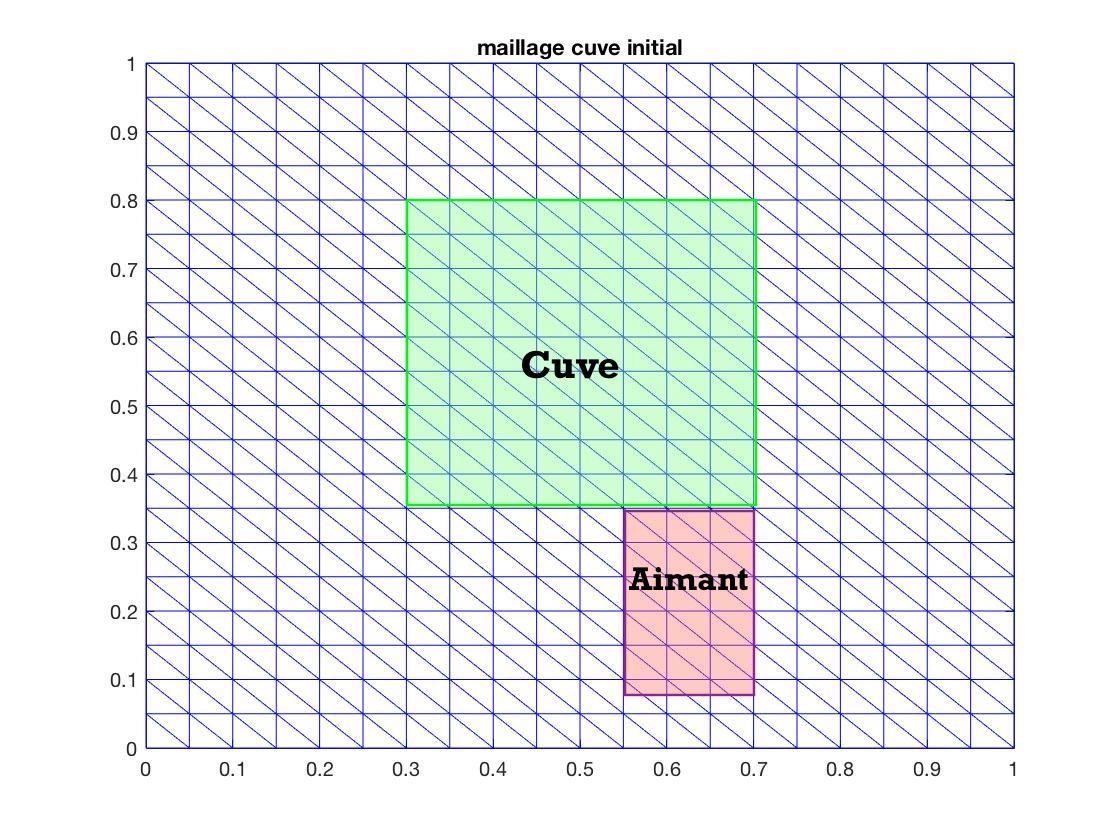
\includegraphics[height = 8 cm, keepaspectratio]{graphes/Maillage_initial1.jpg}
	\caption{affichage résolution centrée sur [-2, 2]}
	\label{figure 1}
	\end{center}
\end{figure}

%===================== implementation algorithmique =======================================
\subsection{Implémentation algorithmique}

Nous allons à présent mettre en place les calculs précédents de manière numérique sur Matlab en maillant le domaine de résolution qui est ici la cuve qui accueille le fluide .  
\\ 
On pose $ L_x,  L_y,  L_z$ les dimensions de la cuve selon x, y, et z.
\newline
Le domaine $\Omega = [0, L_x]\times[0, L_y]\times[0, L_z]$ est ainsi discrétisé par un maillage uniforme défini par les points : 
\\

\[
\left\{
\begin{array}{ccc}
  x_{ij} = (\frac{i\times L_x}{N+1} ,\frac{j\times L_x}{N+1}),    i,j=0,1,......,N+1\\
  y_{ij} = (\frac{i\times L_y}{N+1} ,\frac{j\times L_y}{N+1}),    i,j=0,1,......,N+1  \\
 z_{ij} = (\frac{i\times L_z}{N+1} ,\frac{j\times L_z}{N+1}),    i,j=0,1,......,N+1  
\end{array}
\right.
\]
\begin{figure}[!h]
	\begin{center}
	\centering
		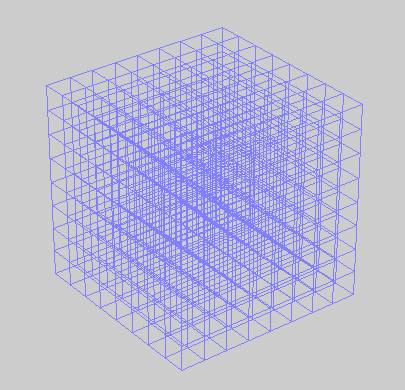
\includegraphics[height = 8cm, keepaspectratio]{graphes/maillage_droit.png} 
		%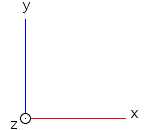
\includegraphics[height = 2cm, keepaspectratio]{graphes/axes.png}
		\caption{maillage du domaine de résolution à l'aide de la fonction matlab $ndgrid$}
	\end{center}
\end{figure}

%============================= calcul champ de vitesse =====================================
\newpage
\subsection{Calcul des matrices du système linéaire}

Pareil qu'avant


%================= implementation algo =============================================================
\subsection{Raccordement à la modélisation du champ magnétique}

Pour résoudre le système linéaire qui découle des équation de Navier-Stokes, nous devons reprendre notre travail précédent pour former le second terme $f$, matrice colonne regroupant les valeurs scalaires de la force magnétique aux différents point du maillage.

Nous devons donc faire le liens entre le maillage de résolution en trois dimension pour la résolutions des équations régissant l'écoulement et le maillage en deux dimensions sur lequel on calcule le champ magnétique. 

Comme nous l'avons énoncé, nous supposons que le champ magnétique est invariant selon le troisième dimensions, il est donc inutile de le recalculer pour chaque 'couche' du maillage 3D, d'autant plus que le maillage 3D est uniforme. 
La méthodologie que nous allons donc appliquer consiste à calculer une unique fois le champ magnétique sur une seule couche de maillage (la couche z = 0 en partique dans l'algorithme) et reprendre les valeurs du champ sur les autres couches.

Ce que nous faisons en pratique est de générer un grand maillage de résolutions 2D pour calculer le champ magnétique, ce qui permet d'atténuer les effets de bord subit par le champ magnétique. 
\newline
Nous utilisons ensuite la fonction Matlab $delaunay$ qui permet à partir du maillage rectangulaire, de définir un maillage triangulaire (comme nous avons travaillé auparavant sur un maillage de type triangulaire quelconque auparavant pour le calcul du champ magnétique).
Nous identifions ensuite sur ce maillage de résolution 2D un domaine correspondant à la cuve est un domaine correspondant à l'aimant, en fonction de la configuration choisie. Le maillage sur le domaine assigné à la cuve doit bien sur correspondre à une couche du maillage de résolution 3D utilisé pour la résolution des équations de Navier-Stokes.

\begin{figure}[!h]
	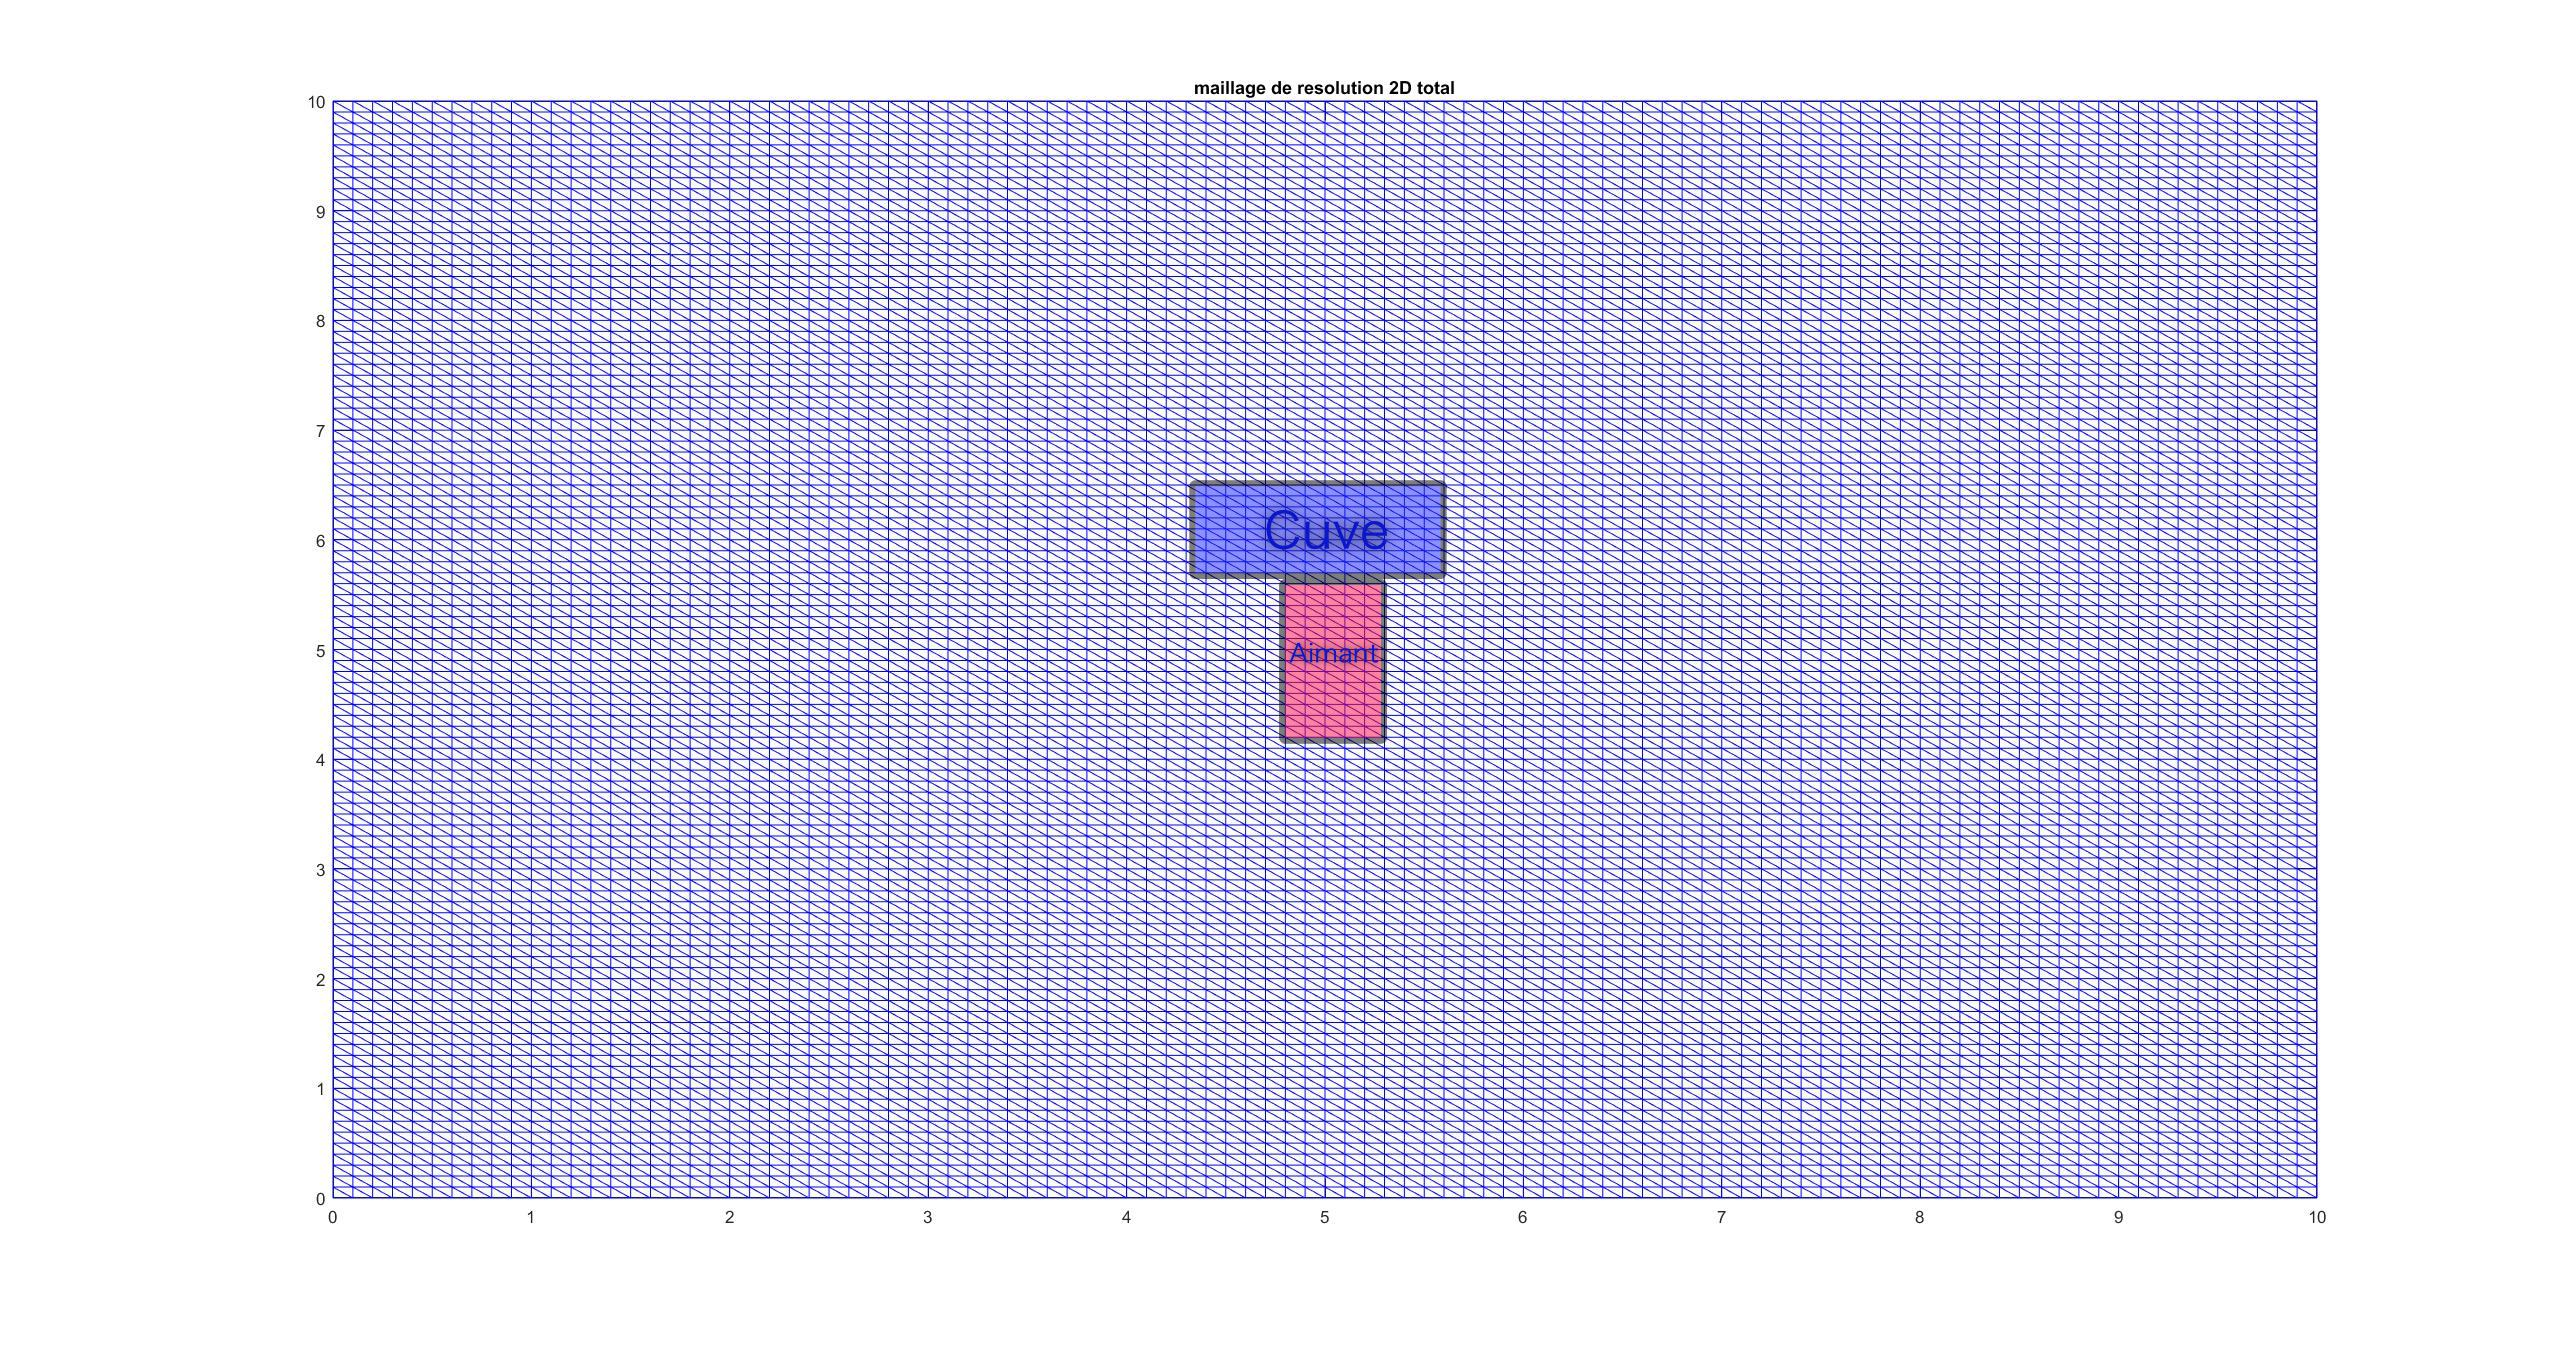
\includegraphics[height = 8cm, keepaspectratio]{graphes/maillage_resolution_total_centre.jpg}
	\caption{\label{figure 3 } configuration dans le cas de la résolution pour la configuration avec l'aimant centré}
\end{figure}
\begin{figure}[!h]
	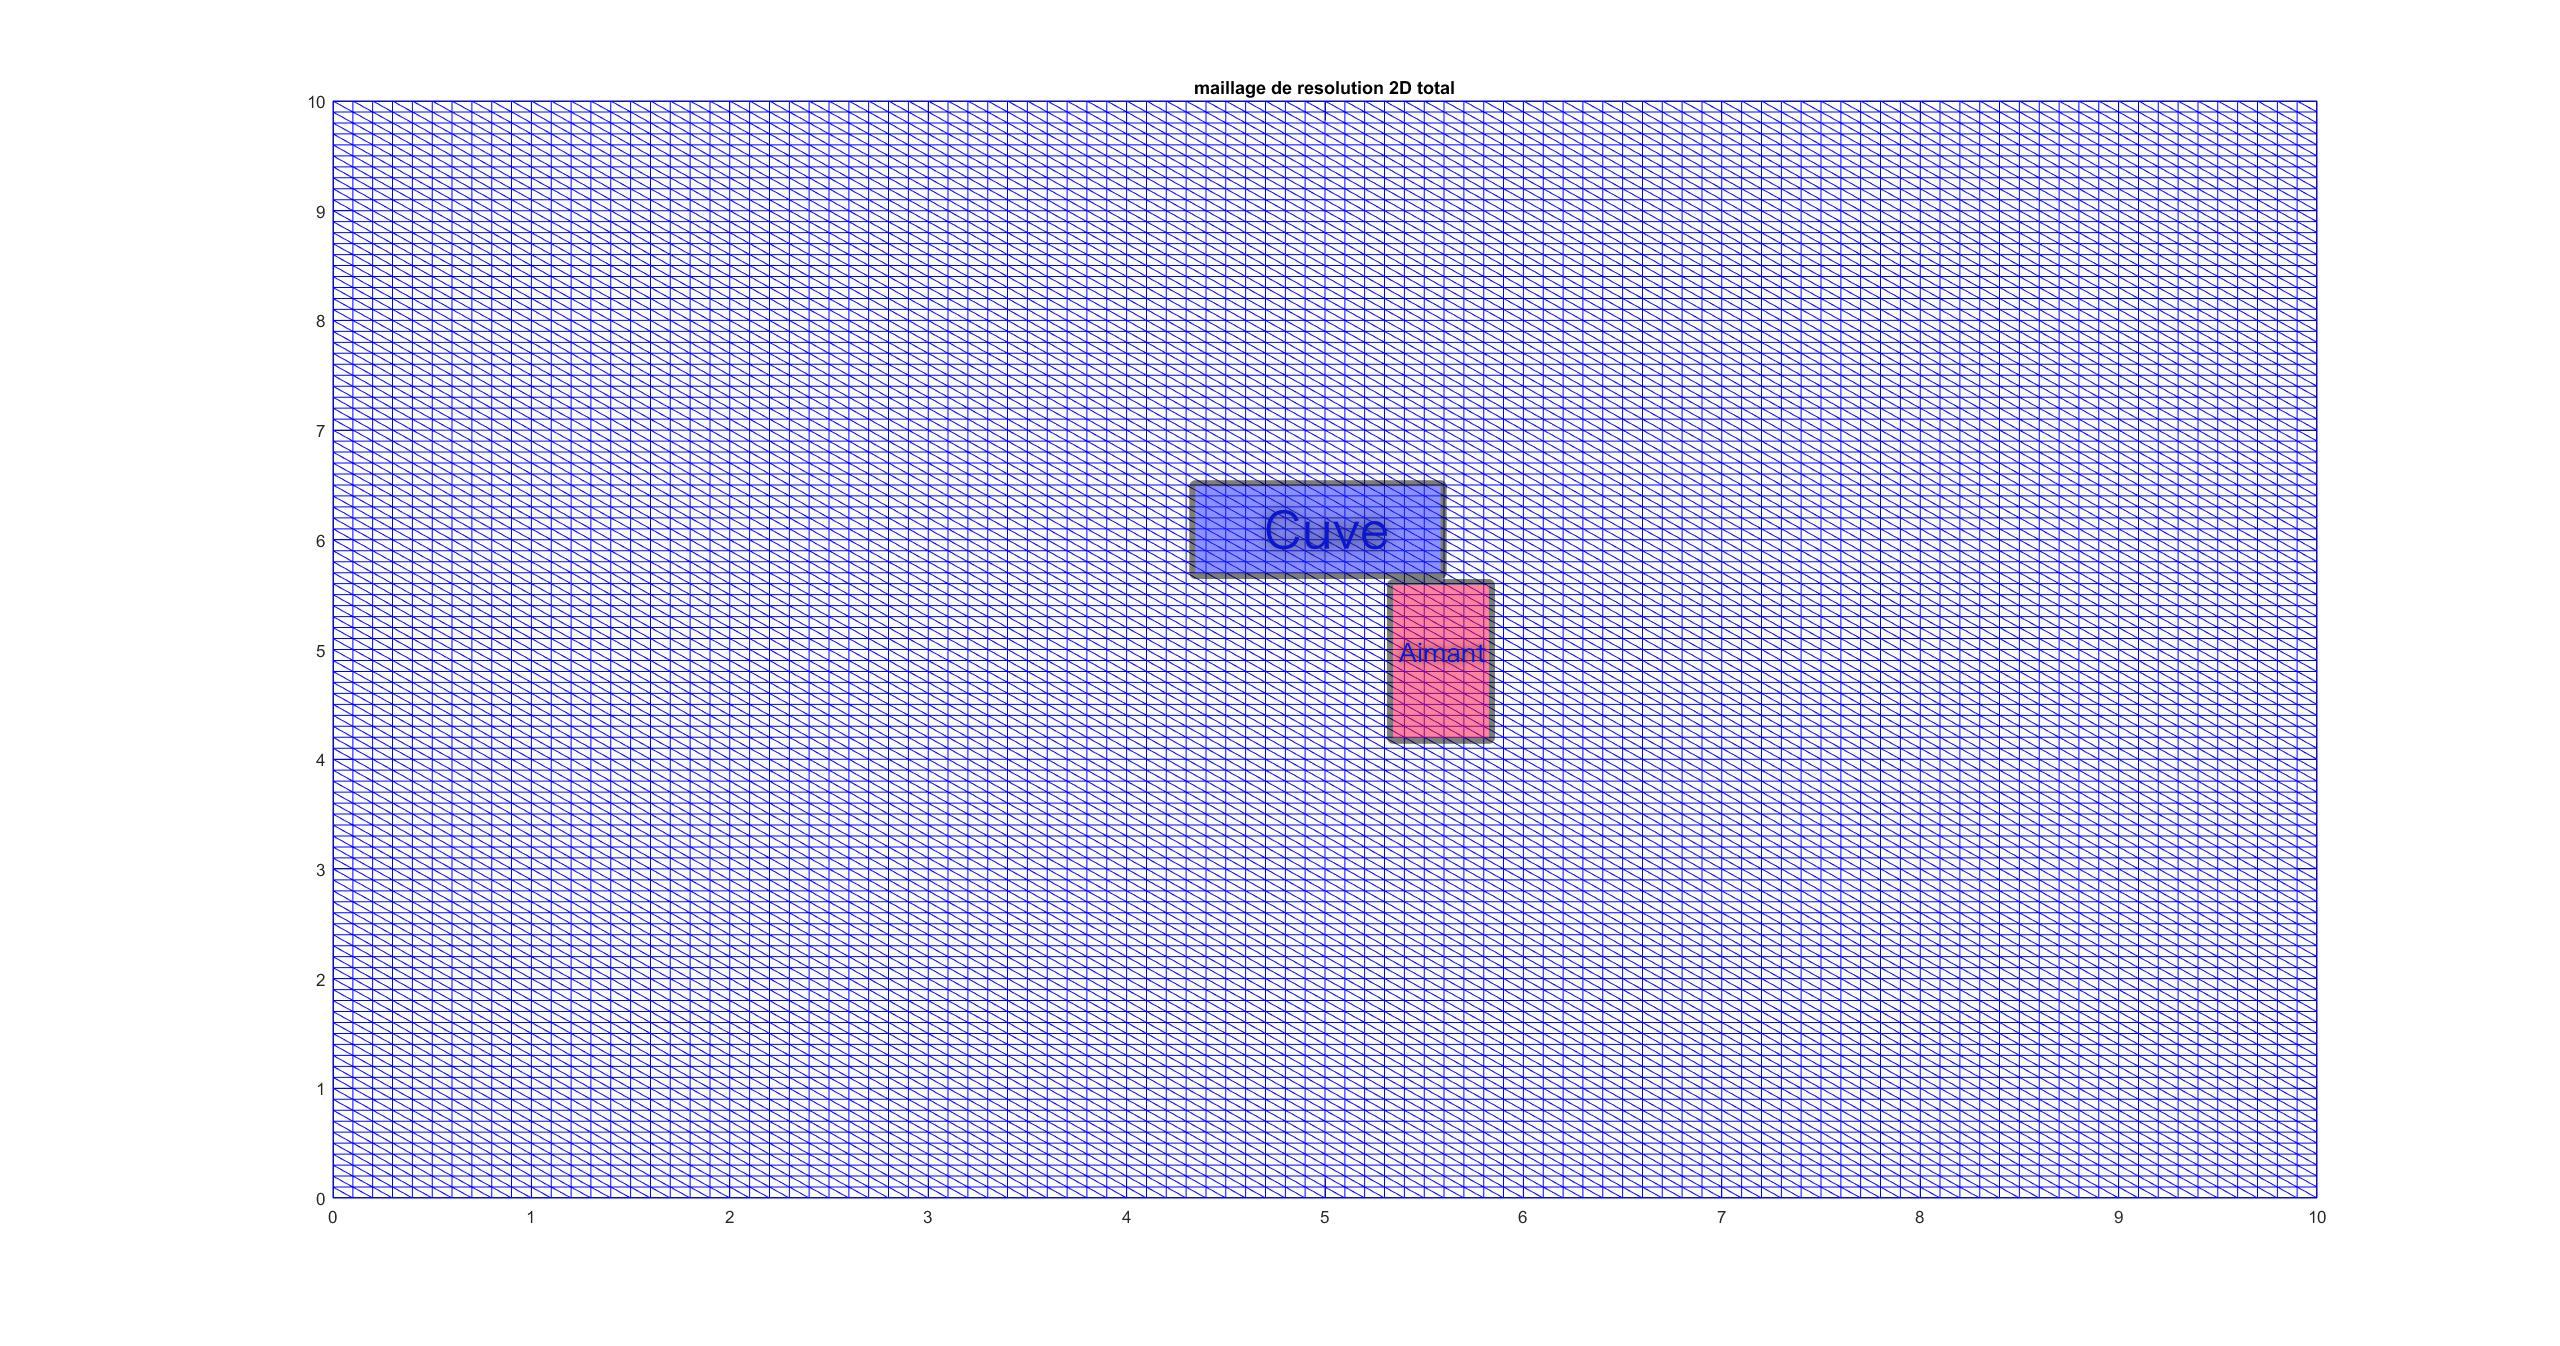
\includegraphics[height = 8cm, keepaspectratio]{graphes/maillage_resolution_total_decentre.jpg}
	\caption{\label{figure 3 } configuration dans le cas de la résolution pour la configuration avec l'aimant décentré}
\end{figure}

\newpage
Algorithmiquement, pour assigner les différents domaines du maillage de résolution 2D généré, nous utilisons le vecteur label $fnum$ qui prend sur chaque triangle la valeur 1, 2, ou 3 en fonction du domaine qui lui a été assigné.
\newline
Maintenant  notre objectif est de pouvoir adapter les données extraites à l'algorithme de Stokes 3D. Le premier obstacle est de réindexer le numéro des triangles pour qu'il y ait une bonne consistance des données lorsque l'algorithme va les utiliser: il faut renuméroter les triangles dans l'ordre. 
\newline  	

Un autre point important est le degré d'interpolation des espace polynomiaux sur lessquels nous travaillons. En effet nous avons résolu les équations du champ magnétique avec des éléments finis de degrés d'interpolation polynomiales 1 (éléments P1), alors que la résolution des équations de Navier-stokes nécessite des éléments finis P2. Il faut donc doubler le nombre de points d'interpolations du champ magnétique avant d'injecter le second membre $f$ dans l'algorithme de résolution des équations de Navier Stokes. Les données prennent alors une nouvelle structure suite à ce dédoublement des point, les matrices ne suivent plus le sens de parcourt des données fixé avec la fonctions de génération de maillage $ngrid$(qui est une généralisation sur la troisième dimension  de $meshgrid$). Ce doublement de point du maillage avec la génération des tables nouvelles tables de descriptions du maillage t et v sont faite par la fonction $mesh_3D$ fournis par M. Scheid que nous utilisons comme une boite noire.

On le voit tout de suite avec un affichage avec un affiche $triplot$ après avoir appliqué $delaunay$ sur les données de la couche 2D du maillage 3D dont on a doublé les points.
\begin{verbatim}
z = 0;   % niveau z = 0
indz = find(v(:,3) == z);		% récupération des indices des nœuds pour le niveau 0
xz = v(indz,1); yz = v(indz,2); vz = [xz, yz];
tz = delaunay(xz,yz);               % triangulation de Delaunay 
triplot(tz,xz,yz);   				% affichage
\end{verbatim}

\begin{figure}[!h]
	\center
	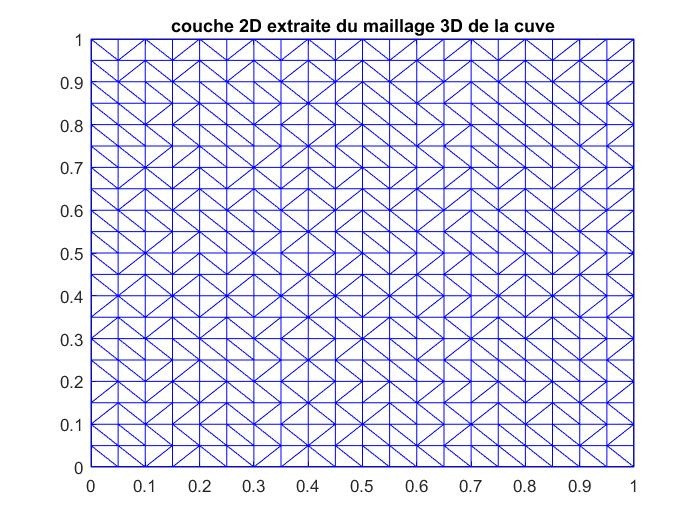
\includegraphics[height = 8cm, keepaspectratio]{graphes/affichage_extraction_2D.jpg}
	\caption{\label{figure 3 } affichage avec $triplot$ du maillage extrait}
\end{figure}
Si on compare à une structure de données classiques généré avec $meshgrid$ ou $linspace$:
\begin{verbatim}
t_total_2D = delaunay(v_total_2D(:,1),v_total_2D(:,2)); 
triplot(t_total_2D ,X_total_2D,Y_total_2D);
xlim([4.5 5.5]);
ylim([4.5 5.5]);
\end{verbatim} 
\begin{figure}[!h]
	\center
	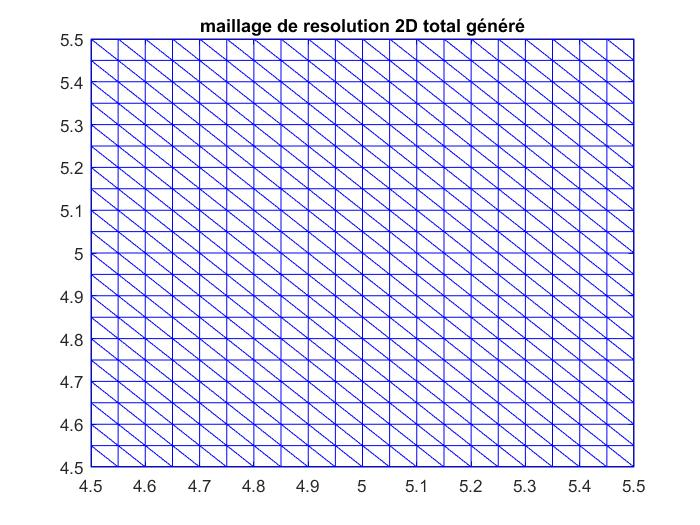
\includegraphics[height = 8cm, keepaspectratio]{graphes/affichage_extraction_2D_normal.jpg}
	\caption{\label{figure 3 } affichage avec $triplot$ du maillage extrait}
\end{figure}
\newpage
Pour comprendre la structure des données il faut alors se rapporter  aux tables de connectivité pour le type de maillage 3D généré.
\begin{figure}[h]
\center
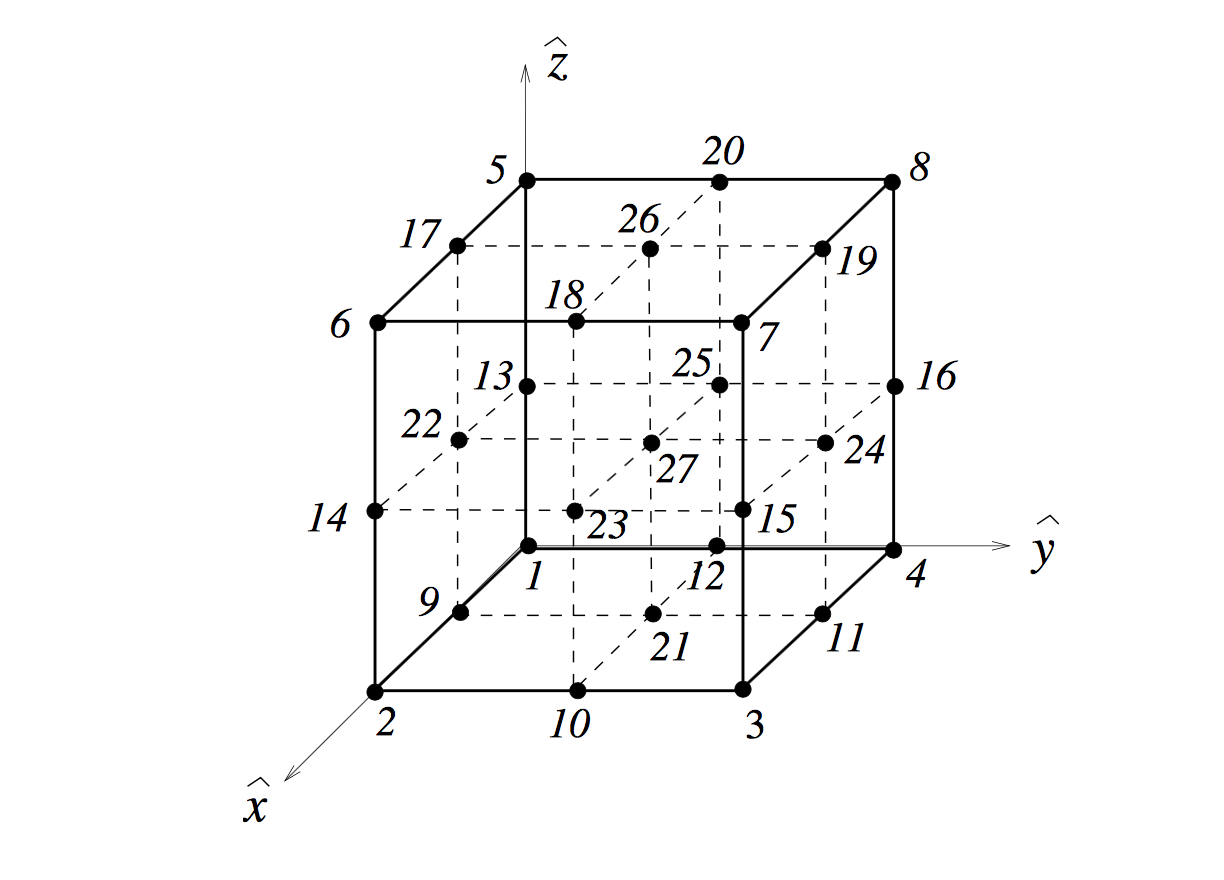
\includegraphics[height = 8cm, keepaspectratio]{graphes/table_de_connectivite.png} 
\caption{\label{figure 3 } table de connectivité, issu du cours $Analyse$ $numérique$ $des$ $équations$ $de$ $Navier$-$Stokes$, J.-F. Scheid}
\end{figure}
On comprend alors que cette structure des données ératique est du à l'arrangement de la tables de coordonnées v. Cela ne pose pas de problème dans la mesure où nous prenons garde à garder la même structure de données tout de long de notre algorithme de résolution est donc d'arranger selon la même structure le second membre $f$.



\newpage
Prenons par exemple les 9 premiers termes de la fonction force de Laplace au niveau $z=0$ à partir de l'origine de ce plan dans le maillage de la cuve. Schématiquement si l'on se limite à la portion $[0;2/N_x].[0;2/N_y]$, on remplit le vecteur $\vec{f_z}$
\\
\[
\vec{f_z}=
\left(
\begin{array}{ccc}
  f_z(0,0) & f_z(1/N_x,0) & f_z(2/N_x ,0)\\
  f_z(0,1/N_y) & f_z(1/N_x,1/N_y) & f_z(2/N_x ,1/N_y) \\
  f_z(0,2/N_y) &  f_z(1/N_x,2/N_y) & f_z(2/N_x,2/N_y )
\end{array}
\right) \overset{\text{selon table de connectivité}}{\Longrightarrow}
\left(
\begin{array}{ccc}
  f_z(0,0)     \\
  f_z(2/N_x ,0)      \\
      f_z(2/N_x,2/N_y )  \\
     f_z(0,2/N_y)\\ 
  ...\\
  f_z(1/N_x,0)\\
   f_z(2/N_x ,1/N_y)\\
   f_z(1/N_x,2/N_y) \\
   f_z(0,1/N_y)\\
   ... \\
    f_z(1/N_x,1/N_y)
\end{array}
\right)
\]
\\
\\
Après formatage du second membre de l'équation à l'algorithme de résolution de Navier Stokes, nous pouvons lancer l'algorithme pour un aimant décentré afin de générer le champ de vitesse dans la cuve. 
Nous pouvons visualiser facilement le champ de vitesse produit par l'algorithme grâce au programme de visualisation physique Paraview: 
voici d'abord le champ de vitesse selon l'axe Y, avec l'aimant centré par rapport à la cuve : 
\begin{figure}[!h]
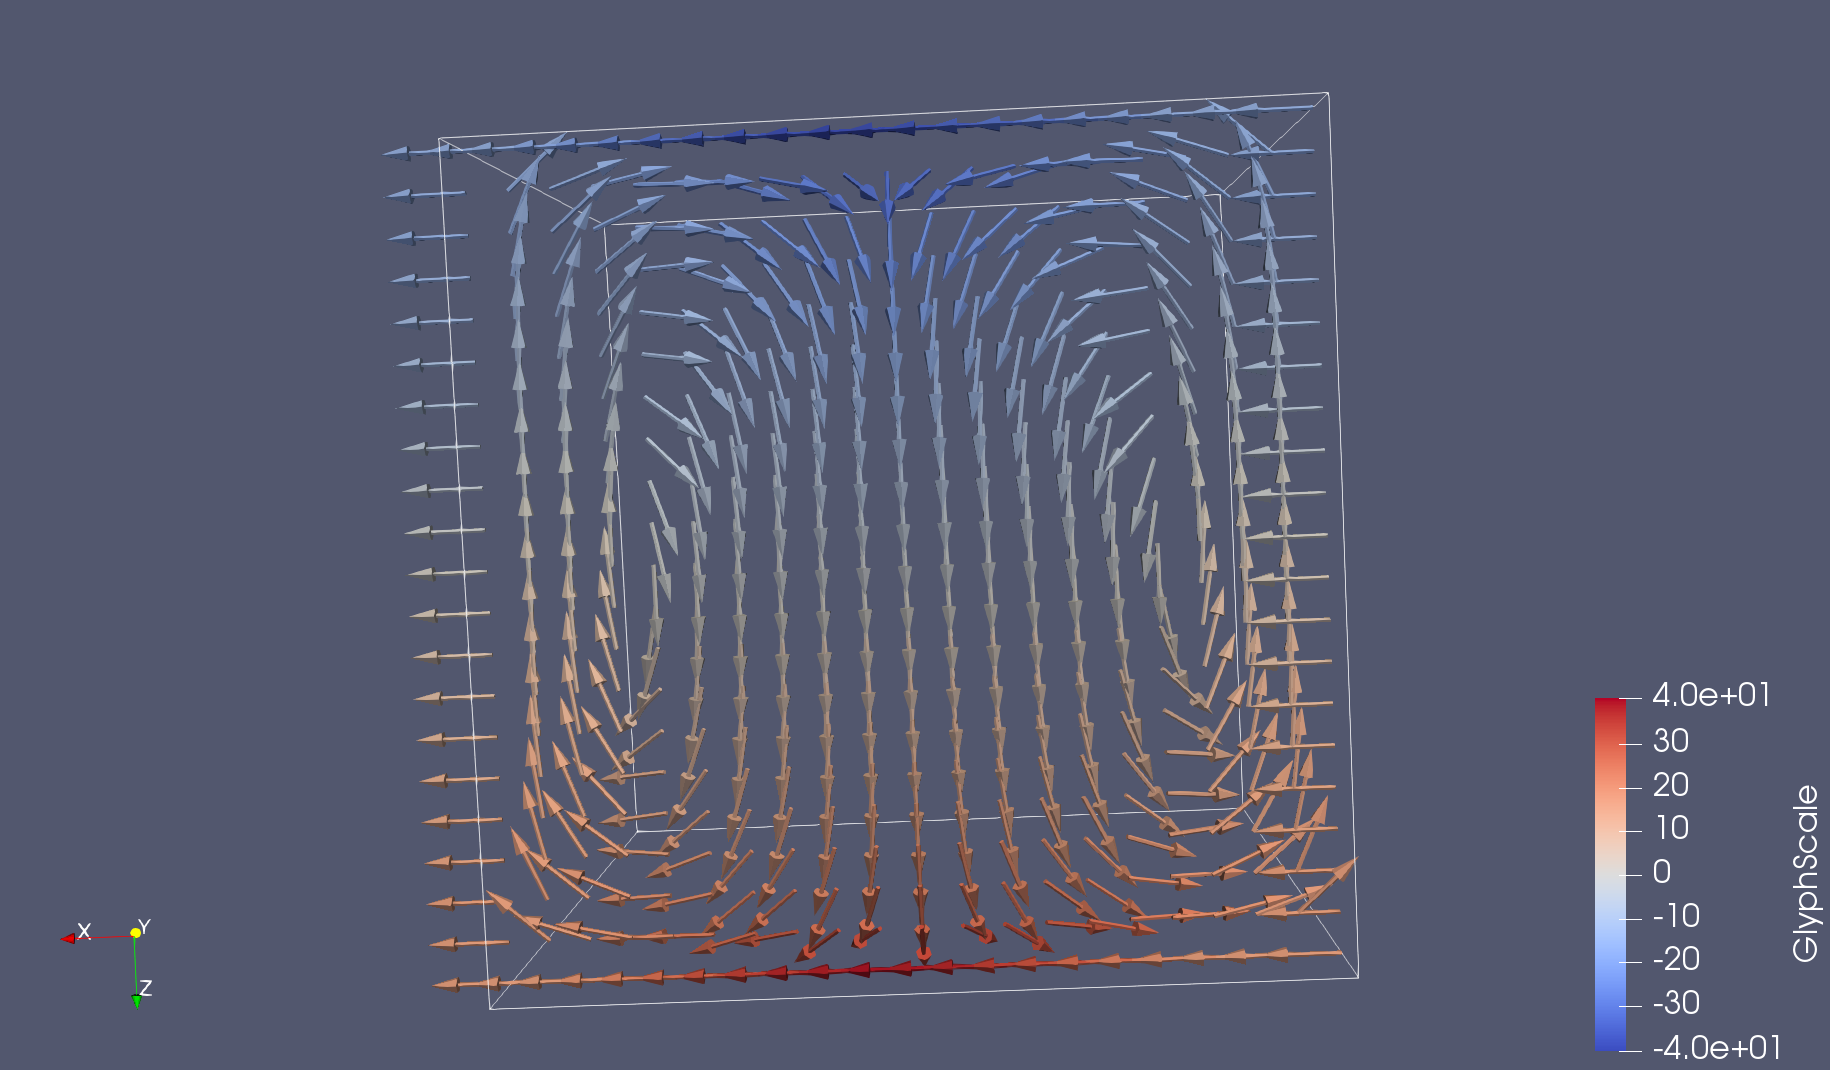
\includegraphics[height = 10cm, keepaspectratio]{graphes/Champ_de_vitesse_selon_Y_centre.png} 
\caption{\label{figure 3 } champ de vitesse obtenue par l'algorithme Stokes3D selon Paraview pour un aimant centré au niveau Y=0}
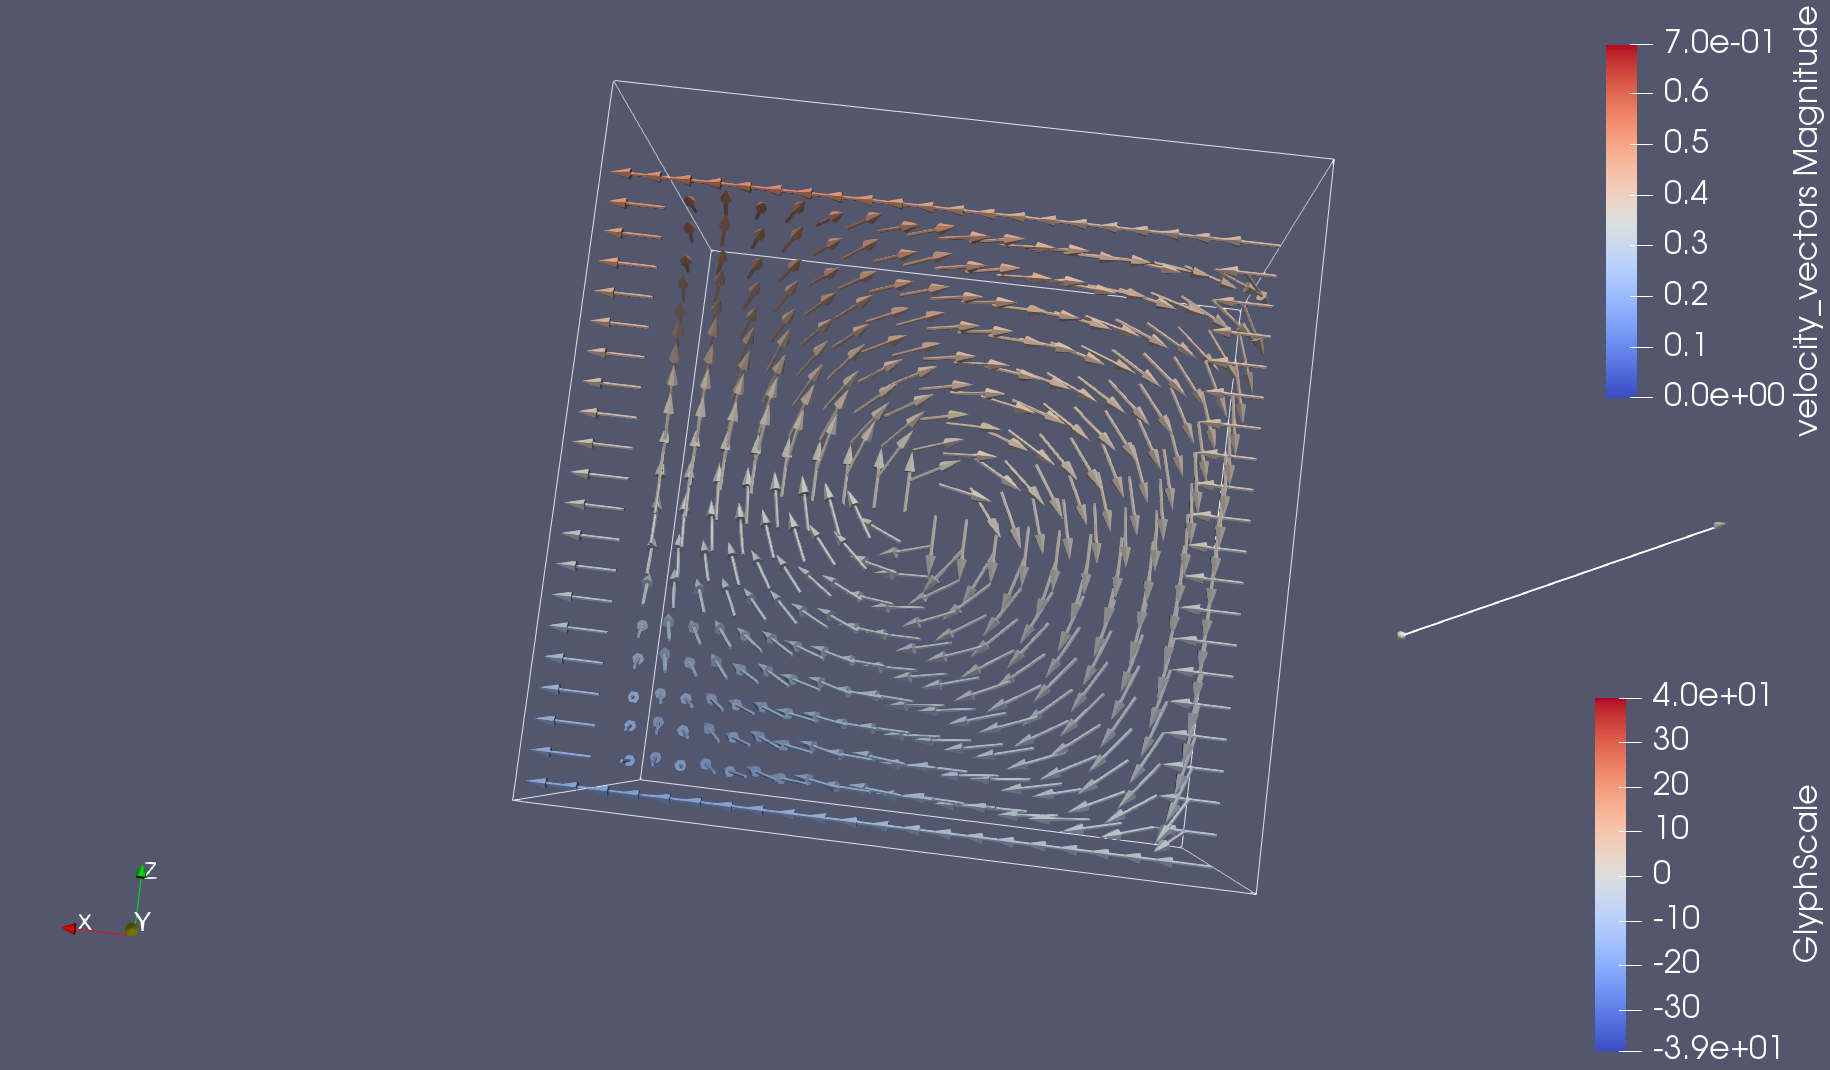
\includegraphics[height = 10cm, keepaspectratio]{graphes/Champ_de_vitesse_selon_Y.png} 
\caption{\label{figure 3 } champ de vitesse obtenue par l'algorithme Stokes3D selon Paraview pour un aimant décentré au niveau Y=0}


\end{figure}
\begin{figure}[!h]

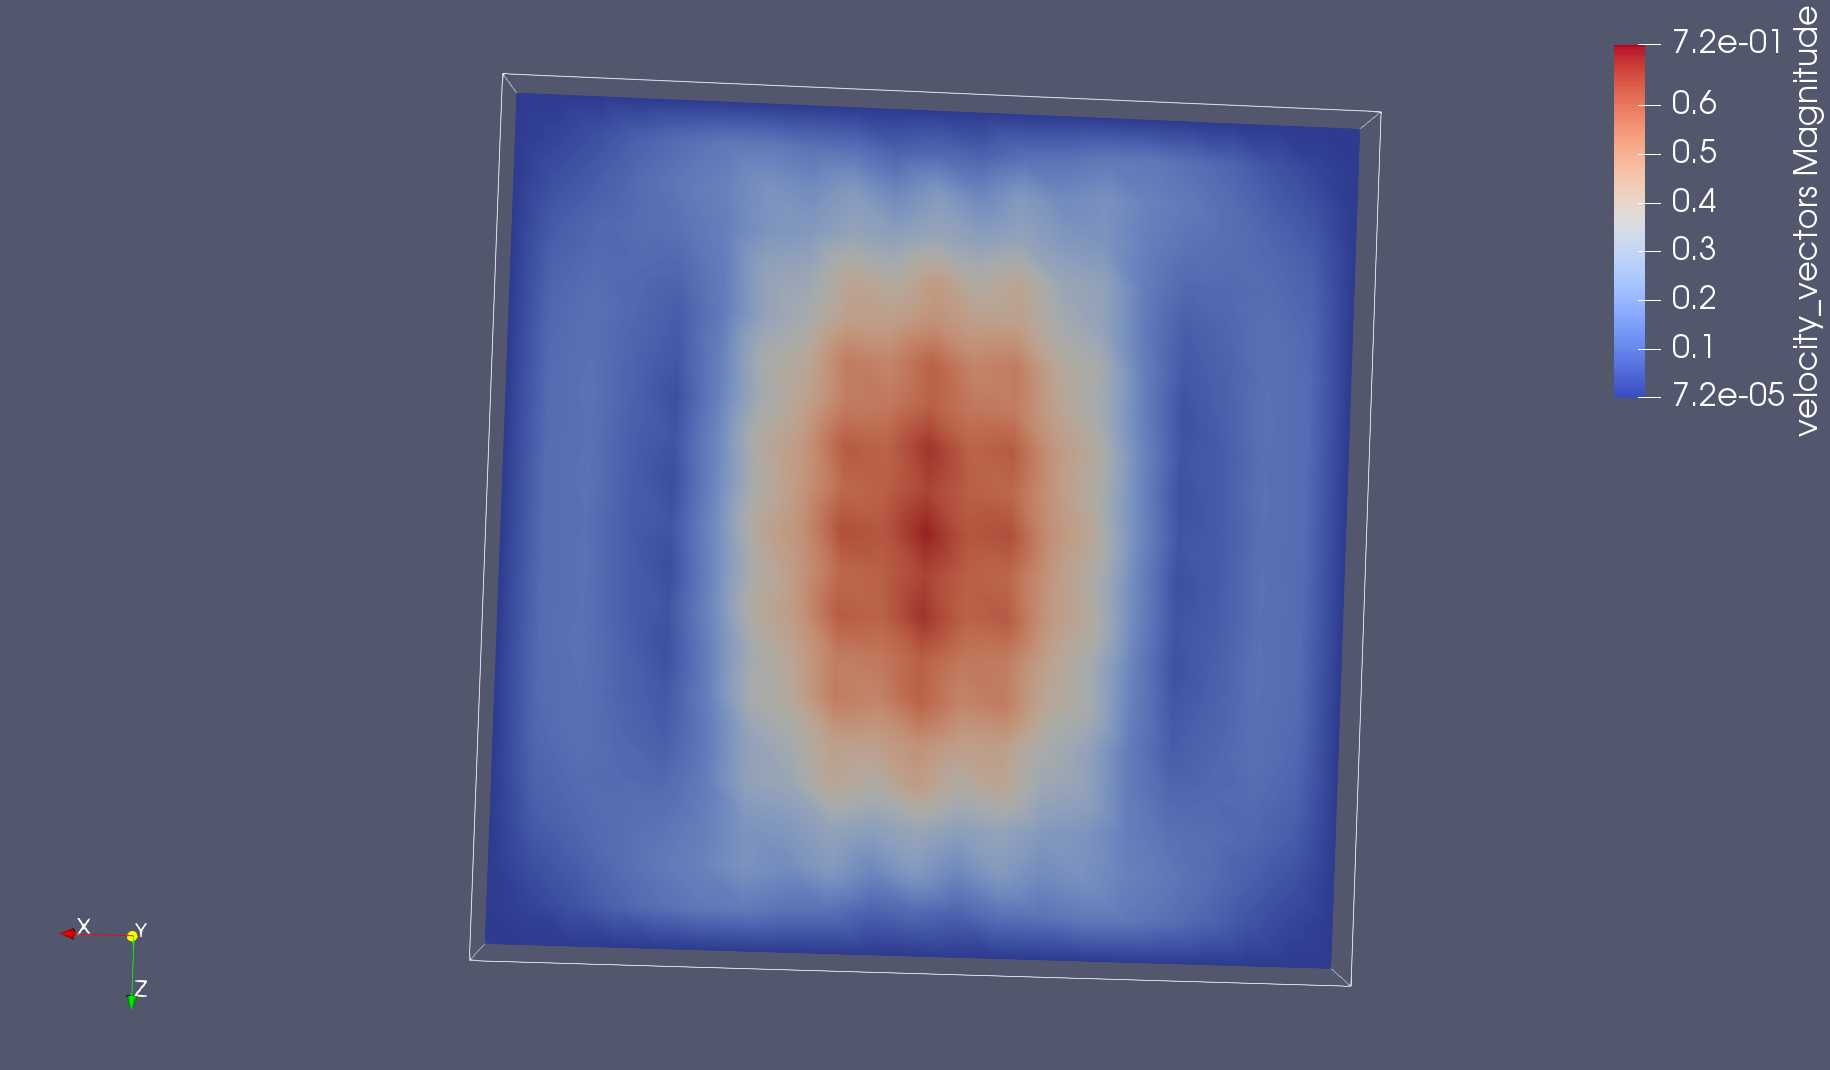
\includegraphics[height = 10cm, keepaspectratio]{graphes/Champ_de_vitesse_selon_Y_centre_ampli.png} 
\caption{\label{figure 3 } champ de vitesse obtenue par l'algorithme Stokes3D selon Paraview pour un aimant centré au niveau Y=0}
%\includegraphics[height = 10cm, keepaspectratio]{graphes/Champ_de_vitesse_selon_Y_decentre_ampli.png} 
\caption{\label{figure 3 } champ de vitesse obtenue par l'algorithme Stokes3D selon Paraview pour un aimant décentré au niveau Y=0}
\end{figure}
nous discernons bien deux lignes de courant pour l'aimant centré, et une ligne de courant pour l'aimant excentré sur le côté selon $\vec{ox}$.


%==========================================================================================================================================================
%														Annexe
%==========================================================================================================================================================

\begin{appendix}

%================================ matrice de rigidité ====================================================================
\chapter{Calcul de la matrice de rigidité}
\label{annexe_1}

La matrice Jacobienne de la transformation est définie par
\[	
J =
\begin{pmatrix}
  \frac{\partial\varphi_{1}}{\partial \hat{x}_{1}} & \frac{\partial\varphi_{2}}{\partial \hat{x}_{2}}  & \frac{\partial\varphi_{3}}{\partial \hat{x}_{1}}\\ 
  \frac{\partial\varphi_{1}}{\partial \hat{x}_{2}} & \frac{\partial \varphi_{2}}{\partial \hat{x}_{2}} & \frac{\partial\varphi_{3}}{\partial \hat{x}_{2}} 
\end{pmatrix} 
\times
\begin{pmatrix}
   x_{1} &  y_{1} \\
   x_{2} &  y_{2} \\
   x_{3} &  y_{3}
\end{pmatrix}
\]
\[
\frac{\partial \hat{\varphi}}{\partial \hat{x}_{1}}(\hat{x}) = 
\frac{\partial}{\partial \hat{x}_{1}}(\varphi(F(\hat{x})) = 
\frac{\partial \varphi}{\partial x_{1}}(x) \frac{\partial F_{1}}{\partial \hat{x}_{1}}(\hat{x}) +
\frac{\partial \varphi}{\partial x_{2}}(x) \frac{\partial F_{2}}{\partial \hat{x}_{1}}(\hat{x})
\]

Donc
\[ \bigtriangledown_{\hat{x}} \hat{\varphi} = 
\begin{pmatrix}
   \frac{\partial F_{1}}{\partial \hat{x}_{1}} & \frac{\partial F_{2}}{\partial \hat{x}_{2}}\\
\end{pmatrix}
\times 
\begin{pmatrix}
   \frac{\partial \varphi}{\partial x_{1}}(x) \\
   \frac{\partial\varphi}{\partial x_{2}}(x)
\end{pmatrix} = 
J^{T} \times \bigtriangledown_{x} \varphi \]

Calculons $\bigtriangledown_{\hat{x}} \hat{\varphi}$ sur le triangle de référence $\hat{T}$ :
\[
\left\{
\begin{array}{ccc} 
	\begin{aligned}
		\hat{\varphi}_{1} &= -\hat{x}_{1}+1-\hat{x}_{2} \\  %\qquad 	
		\hat{\varphi}_{2} &= \hat{x}_{1}                \\  %\qquad 
		\hat{\varphi}_{3} &= \hat{x}_{2}
	\end{aligned}
\end{array}
\right.
\]
En effet $\hat{\varphi}_{1}$ vaut 1 sur le sommet 1 et 0 sur les autres sommets (Figure 3).
Ainsi
\[ \bigtriangledown_{\hat{x}} \hat{\varphi}_{1} = 
\begin{pmatrix}
   -1 \\
   -1
\end{pmatrix}
\qquad
\bigtriangledown_{\hat{x}} \hat{\varphi}_{2} = 
\begin{pmatrix}
   -1 \\
   -1
\end{pmatrix}
\qquad
\bigtriangledown_{\hat{x}} \hat{\varphi}_{1} = 
\begin{pmatrix}
   -1 \\
   -1
\end{pmatrix}
\]
et donc
\[
\bigtriangledown_{\hat{x}} \hat{\varphi}(\hat{x}) = 
\begin{pmatrix}
   -1 & 1 & 0 \\
   -1 & 0 & 1 
\end{pmatrix}
\]
\[	
J =
\begin{pmatrix}
   -1 & 1 & 0 \\
   -1 & 0 & 1 
\end{pmatrix}
\times
\begin{pmatrix}
   x_{1} &  y_{1} \\
   x_{2} &  y_{2} \\
   x_{3} &  y_{3}
\end{pmatrix} =
\begin{pmatrix}
   x_{2}-x_{1} &  y_{2}-y_{1} \\
   x_{3}-x_{1} &  y_{3}-y_{1}
\end{pmatrix}
\]
Finalement,
\[
\begin{vmatrix}
   J
\end{vmatrix}
= (x_{2}-x_{1})\times (y_{3}-y_{1})-(x_{3}-x_{1})\times(y_{2}-y_{1})= 2\times\text{Aire}(T)
\]
où $|J|$ est le déterminant de la matrice $J$
et ainsi
\[ \bigtriangledown_{x} \varphi =  (J^{-1})^{T} \times \bigtriangledown_{\hat{x}} \hat{\varphi} \]
avec
\[
J^{-1} =  \frac{1}{|J|}
\begin{pmatrix}
   J_{22} & -J_{12} \\
   -J_{21} & J_{11}
\end{pmatrix}
\]
d'où
\[
*\begin{aligned}
	(J^{-1})^{T} 
	&=  	
	\frac{1}{|J|}
	\begin{pmatrix}
   		J_{22} & -J_{21} \\
   		-J_{12} & J_{11}	
	\end{pmatrix} \\
	&=
	\frac{1}{2\times \text{aire}(T)}
	\begin{pmatrix}
   		J_{22} & -J_{21} \\
   		-J_{12} & J_{11}	
	\end{pmatrix} 
	\end{aligned}
\]

Et le calcul du terme $A_{ij}$ de la matrice de rigidité, on obtient ainsi avec le changement de variable vers le triangle de référence.
\[
\begin{aligned}
	\text{A}_{ij} 
	&=
	\sum_{T \in \text{Supp}(\varphi_{i})\times \text{Supp}(\varphi_{j})} 
	\iint_{(i,j) \in T}\bigtriangledown_{x}{\varphi_{i}} \bigtriangledown_{x}{\varphi_{j}} \\
	&=
	\sum_{T \in \text{Supp}(\varphi_{i})\times \text{Supp}(\varphi_{j})}
	\iint_{(i,j) \in T} (J^{-1})^{T}|J|(J^{-1})^{T}|J|
	\times
	\bigtriangledown_{\hat{x}} \hat{\varphi_{i}}
	\times
	\bigtriangledown_{\hat{x}} \hat{\varphi_{j}} \\
	&=
	\sum_{T \in \text{Supp}(\varphi_{i})\times \text{Supp}(\varphi_{j})}	
	\frac{\text{aire}(T)^{2}}{4}
	\begin{pmatrix}
   		y_{3}-y_{1} &  	x_{1}-x_{3}\\
   		y_{1}-y_{2} &  x_{2}-x_{1}
	\end{pmatrix}
	^{2}
	\bigtriangledown_{\hat{x}} \hat{\varphi_{i}}
	\bigtriangledown_{\hat{x}} \hat{\varphi_{j}}
\end{aligned}
\]

%================================= CODE MATLAB ===========================================================================

\chapter{Codes Matlab}
\label{annexe_2}

\subsection{Modélisation du champ magnétique}









\iffalse
%==========================================================================================================================================================	
\chapter{Démonstration de l'existence d'une solution u}
%==========================================================================================================================================================
\label{Démonstration 1}
On a : 
\[
\left \{
\begin{array}{ccc}
  \Div\vec{B} = 0   &   \\
  \vec{B} = \mu_{0}\times(\vec{grad} +\vec{M}) \\
  \vec{M_{0} } \ sur \  \Omega_{i}  \ et \ \vec{0}  \ sur \  \Omega_{e}
\end{array}
\right .
 \iff \ \left\{\begin{array}{cc} -\Delta u= -div(\vec{M})=0 \ sur\ \Omega \\ \\u \ = \ 0 \ sur \ \partial \Omega \end{array}\right.
\]
\\
donc au sens des distributions , $\forall \varphi \in D(\Omega)$ 
\[
\begin{aligned}
<-\Delta u,\varphi> &=  0 \\
\iff \sum_{k=1}^{3} <  \frac{\partial u}{\partial x_{k}}, \frac{\partial \varphi}{\partial x_{k}}> &= 0
\end{aligned}
\]
\\
Or u $\in H^{1}_{0}(\Omega)$ donc $ \frac{\partial u}{\partial x_k} \in L^{2}(\Omega)$
\\
donc $<  \frac{\partial u}{\partial x_k}, \frac{\partial \varphi}{\partial x_k}>=\int_{\Omega} \frac{\partial u}{\partial x_k} \times \frac{\partial \varphi}{\partial x_k}\, \mathrm{d}x $
\\
donc le probleme peut s'établir ainsi: $<\bigtriangledown u ,\bigtriangledown \varphi>_{L^{2}(\Omega) }= 0 ,\ \forall \varphi \in D(\Omega) $
\\
Or on sait que l'ensemble $\Omega$ est bornée dans au moins une direction 
\\
donc on peut écrire $< u,\varphi>_{H^{0}_{1}(\Omega)}=0 \ \forall \varphi \in D(\Omega) $
\\
 0 est une forme lineaire continue pour n'importe quelle espace vectoriel 
 \\ donc d'apres le théorème de représentation de Riesz, dans $H^{0}_{1}(\Omega)$,
\\
$\exists ! u_{0} \in H^{0}_{1}(\Omega)$ telle que $<u_{0},v>_{H^{0}_{1}(\Omega)}=0,\ \forall v\in {H^{0}_{1}(\Omega)} $

Pour trouver le champ magnétique, on appliquer les équations fondamentales de la magnétostatique. L'équation de Maxwell nous donne 
\[
\begin{aligned}
\Rot{\vec{H}} &= \vec {0} \\
\Div{\vec{B}} &= 0
\end{aligned}
\]

Le domaine étant simplement connexe, $\vec{H}$ dérive d'un potentiel U.
\[\vec{H}= \Grad{\vec{U}}\]
\[\vec{B} = \mu_{0}\times(\vec{\Grad{U}}+\vec{M})\]

Au sens des distributions pour toute fonction $\varphi\ $ dans $D(\Omega)$
\[<\Div\vec{B},\varphi> =  <-\vec{B},\vec{\Grad{\varphi}}>\]
On suppose $\vec{B} \in L^{3}_{1}(\Omega)$
\[<\Div\vec{B},\varphi> =  -\int_{\Omega}\vec{B}. \vec{\Grad{\varphi}}\]
\[<\Div\vec{B},\varphi> =  -\int_{\Omega}\mu_{0}(\vec{\Grad{U}}+\vec{M}) .{\Grad{\varphi}} = 0\]
Ainsi
\[\int_{\Omega}(\vec{\Grad{U}}+\vec{M}) . \vec{\Grad{\varphi}} = 0\]
Et comme $\vec{M}$ est nul en dehors du domaine $\Omega_{\text{int}}$ de l'aimant, on obtient (1)
\fi



\iffalse
%==========================================================================================================================================================
\chapter{Démonstration équation (1)}
%==========================================================================================================================================================
\label{Démonstration 2}	
	Pour trouver le champ magnétique, on appliquer les équations fondamentales de la magnétostatique. L'équation de Maxwell nous donne 
	\[
		\left\{
		\begin{array}{ccc}
			\begin{aligned}
				\Rot{\vec{H}} &= \vec {0} \\
				\Div{\vec{B}} &= 0
			\end{aligned}
		\end{array}
		\right.
	\]

	Le domaine étant simplement connexe, $\vec{H}$ dérive d'un potentiel $u$	.
	\[
		\left\{
		\begin{array}{ccc}		
		\begin{aligned}
			\vec{H} &= \Grad{\vec{u}} \\
			\vec{B} &= \mu_{0}\times(\vec{\Grad{u}}+\vec{M})
		\end{aligned}
		\end{array}
		\right.
	\]

	Au sens des distributions pour toute fonction $\varphi\ $  dans $D(\Omega)$	
	\[<\Div\vec{B},\varphi> \ = \ <-\vec{B},\vec{\Grad{\varphi}}>\]
	On suppose $\vec{B} \in L^{3}_{1}(\Omega)$
	\[<\Div\vec{B},\varphi> \ = \  -\int_{\Omega}\vec{B}. \vec{\Grad{\varphi}}\]
	\[<\Div\vec{B},\varphi> \ = \ -\int_{\Omega}\mu_{0}(\vec{\Grad{u}}+\vec{M}) .{\Grad{\varphi}} = 0\]
	Ainsi
	\[\int_{\Omega}(\vec{\Grad{u}}+\vec{M}) . \vec{\Grad{\varphi}} = 0\]
	Et comme $\vec{M}$ est nul en dehors du domaine $\Omega_{\text{int}}$ de l'aimant, on obtient (1)
	%je rentre l'equation on pourra y faire appel plus tard avec \ref{E}
	\[
		\forall \varphi\ \in \Omega, \ \int_{\Omega}\vec{\Grad{u}}.\vec{\Grad{\varphi}} = -\vec{M_{0}}. \int_{\Omega_{int}}\vec{\Grad{\varphi}}
	\]
\fi

\end{appendix}
\end{onehalfspace}

\newpage
\Large \bf Bibliographie

\mdseries  "Introduction à l'analyse numérique"(1998), de Jacque Rappaz et Marco Picasso, publié par les Presses polytechniques et universitaires romandes.
\\
\\
"Méthode des éléments finis : élasticité plane" par Yves Dabard, Institut Universitaire de Technologie du Mans Département Génie Mécanique et Productique
, http://iut.univ-lemans.fr/ydlogi/index.html, 24 mars 2006 – 29 mars 2011
%
%" par un écoulement stationnaire de fluide à faible Reynolds", par Ismail Mebsout et Oumaima Hammami, 2017,  Institut ´ Elie Cartan de Lorraine.
%
\\
\\
\mdseries "Analyse numérique des équations de Navier-Stokes",de Jean-François Scheid,  Cours de Master 2 Mathématiques (Recherche) - Université de Lorraine, Nancy.
\\
\\
\mdseries "Projet de deuxième Année : Génération de maillages 2D avec Matlab" de Jean-Philippe LEBOUCHER Benjamin PACCOU avec comme chef de Projet Jonas KOKO, Institut
Supérieur d’ Informatique, de Modélisation et de leurs Applications
\bibliographystyle{plain}
\bibliography{bibli}




 



\end{document}








